\documentclass[UTF8]{ctexart}
\usepackage[a4paper, margin=2.2cm]{geometry}
\usepackage{graphicx}
\usepackage{float}
\usepackage{booktabs}
\usepackage{longtable}
\usepackage{array}
\usepackage{multirow}
\usepackage{tabularx}
\usepackage{enumitem}
\usepackage{amsmath}
\usepackage{amssymb}
\usepackage{xcolor}
\usepackage{hyperref}
\usepackage{caption}
\usepackage{subcaption}
\usepackage{tikz}
\usepackage{listings}
\usepackage{fancyhdr}
\usetikzlibrary{arrows.meta, positioning, shapes.geometric, calc}

\hypersetup{
  colorlinks=true,
  linkcolor=blue!55!black,
  urlcolor=blue!55!black,
  citecolor=blue!55!black
}

\pagestyle{fancy}
\setlength{\headheight}{15pt}
\fancyhf{}
\lhead{Google Play 年龄分级问卷逆向建模}
\rhead{社交隐私网络大作业}
\cfoot{\thepage/\pageref{LastPage}}

\lstdefinestyle{code}{
  basicstyle=\ttfamily\small,
  breaklines=true,
  columns=fullflexible,
  frame=single,
  rulecolor=\color{black!20},
  backgroundcolor=\color{black!3},
  showstringspaces=false,
  tabsize=2
}
\lstset{style=code}

\newcommand{\code}[1]{\texttt{\footnotesize\detokenize{#1}}}
\newcommand{\projecttitle}{Google Play 年龄分级问卷的黑盒逆向建模与预测}
\newcommand{\repo}{CYH0415/OSN-Lab-Main}

\begin{document}

\begin{titlepage}
\centering
\vspace*{1.0cm}

\includegraphics[width=0.78\textwidth]{figures/head.png}

\vspace{1.8cm}

\includegraphics[width=0.24\textwidth]{figures/badge.png}

\vspace{1.6cm}
{\zihao{2}\bfseries 社交隐私网络课程大作业报告\par}
\vspace{0.7cm}
{\zihao{3}\bfseries \projecttitle\par}

\vfill
\begin{center}
\zihao{4}
\renewcommand{\arraystretch}{1.6}
\begin{tabular}{rl}
小组成员： & 陈博凡、陈宇涵、陈子涵、史家顺、王子轩 \\
项目仓库： & \url{https://github.com/CYH0415/OSN-Lab-Main} \\
实验对象： & Google Play / IARC 内容分级问卷 \\
预测目标： & 北美地区 ESRB 年龄分级 \code{rating__north_america} \\
核心方法： & 自动化采样、数据清洗、特征工程、多分类机器学习、模型解释分析 \\
\end{tabular}
\end{center}

\vspace{1.2cm}
{\zihao{4}\today\par}
\end{titlepage}

\clearpage
\tableofcontents
\clearpage

\section{摘要}

Google Play 的年龄分级机制用于帮助家长和普通用户判断应用是否适合未成年人使用。开发者在 Google Play Developer Console 中填写 IARC 内容分级问卷后，系统会生成年龄分级、内容描述符和互动元素等结果。然而，Google 并未公开问卷答案到最终分级之间的具体判定规则；开发者和用户只能观察输入问卷答案与输出分级结果，无法直接获知每个问题、每条分支和每类风险内容对最终分级的影响。因此，本项目将 Google Play 年龄分级问卷视为一个黑盒系统，通过自动化采样与机器学习方法逆向建模“问卷答案 $\rightarrow$ 最终年龄分级”的映射关系。

围绕课程要求，本项目完成了树状问卷结构解析、自动化样本提交、数据清洗与验证、特征工程、多模型训练、模型性能比较和分级机制分析。最终数据集中包含 1265 条有效样本，覆盖 All Other App Types、Game、Social or Communication 三类应用问卷分支；清洗后数据被确定性划分为 1012 条训练样本和 253 条测试样本。特征工程阶段将 165 个原始输入字段编码为 758 维模型特征，其中 133 个 radio / categorical 字段采用 one-hot 编码，32 个 checkbox 字段采用 multi-hot 编码，并显式保留 \code{__INACTIVE__}、\code{__NOT_APPLICABLE__}、\code{__NONE__} 等结构性缺失标记。

模型训练阶段共比较了四类模型：L1 正则化 Logistic Regression、Random Forest、LightGBM 和 XGBoost。实验结果显示，L1 正则化 Logistic Regression 在测试集上取得最佳表现：Accuracy 为 0.921，Macro F1 为 0.918，Macro AUC 为 0.977；XGBoost 以 0.814 Accuracy 和约 0.810 Macro F1 排名第二；Random Forest 经调参后达到 0.783 Accuracy 和 0.797 Macro F1；LightGBM 在本数据规模和高维稀疏特征设定下表现相对较弱，Accuracy 为 0.680。进一步分析表明，Google Play 年龄分级主要受血腥/暴力程度、性内容与裸露、药物引用、赌博与现金奖励等高风险问题影响；同时，问卷分支结构本身也携带重要信息，某些问题是否被激活已经隐式反映了风险路径。

本报告详细说明了项目的实验背景、作业要求响应、系统架构、数据采集策略、数据质量控制、特征构造、模型训练与调参、结果分析、遇到的问题及解决方案，并总结了小组分工和后续改进方向。

\section{作业要求与完成情况}

\subsection{作业任务理解}

根据课程项目说明，本选题要求围绕 Google Play 年龄分级问卷完成黑盒逆向建模。作业核心要求可以概括为四部分：

\begin{enumerate}[leftmargin=2em]
  \item \textbf{数据收集策略设计与实现}：针对树状结构的内容分级问卷设计系统、高效的采样策略，并通过脚本自动提交问卷和收集分级结果，至少获得 1000 条有效且具有足够多样性的样本。
  \item \textbf{模型训练与预测}：对采集数据进行特征工程，训练多分类年龄分级预测模型，至少尝试三种不同模型，并进行性能比较与优化。
  \item \textbf{结果分析}：分析整体模型效果、不同年龄分级类别之间的预测差异，探索 Google Play 分级机制中可能存在的规律，例如最具影响力的问题或内容风险因素。
  \item \textbf{完整报告}：报告应覆盖数据收集策略、数据集分析、模型训练、性能评估、问题与解决方案、主要发现、核心代码和关键图表。
\end{enumerate}

本项目的实现不只是对现成数据进行建模，而是从问卷页面自动化探测开始，逐步构建可复现的数据闭环。整体流程如图~\ref{fig:workflow} 所示。

\begin{figure}[H]
\centering
\begin{tikzpicture}[
  node distance=0.72cm,
  flowstep/.style={rectangle, rounded corners=2pt, draw=black!55, fill=blue!5, minimum width=2.55cm, minimum height=1.15cm, align=center, font=\small},
  arrow/.style={-{Latex[length=2.2mm]}, thick, draw=black!65}
]
\node[flowstep] (a) {问卷结构\\自动探测};
\node[flowstep, right=of a] (b) {树状分支\\采样设计};
\node[flowstep, right=of b] (c) {Play Console\\自动提交};
\node[flowstep, right=of c] (d) {数据清洗\\质量验证};
\node[flowstep, below=of d] (e) {特征工程\\758维编码};
\node[flowstep, left=of e] (f) {模型训练\\四类模型};
\node[flowstep, left=of f] (g) {性能评估\\混淆矩阵};
\node[flowstep, left=of g] (h) {机制解释\\结论总结};
\draw[arrow] (a) -- (b);
\draw[arrow] (b) -- (c);
\draw[arrow] (c) -- (d);
\draw[arrow] (d) -- (e);
\draw[arrow] (e) -- (f);
\draw[arrow] (f) -- (g);
\draw[arrow] (g) -- (h);
\end{tikzpicture}
\caption{项目端到端实验流程。项目从动态问卷结构探测开始，经过采样、采集、清洗、编码、建模和解释分析形成闭环。}
\label{fig:workflow}
\end{figure}

\subsection{完成情况总览}

\begin{table}[H]
\centering
\caption{作业要求完成情况对照}
\label{tab:requirements}
\renewcommand{\arraystretch}{1.35}
\begin{tabularx}{\textwidth}{p{3.2cm} X p{2.2cm}}
\toprule
要求 & 项目完成情况 & 状态 \\
\midrule
树状问卷理解 & 使用 Playwright / Chrome CDP 探测三类问卷的题目、选项、父子依赖和分支路径，输出 \code{question_graph.json}、\code{question_graph.md}、\code{question_graph.html} 等结构化产物。 & 已完成 \\
自动化数据采集 & 编写 \code{inspect_questionnaire.mjs}、\code{run_rating_samples.mjs}、\code{autonomous_rating_sampler.mjs} 等脚本，能够复用真实 Chrome 登录态，在 Google Play Console 自动填写、提交、解析并保存分级结果。 & 已完成 \\
至少 1000 条有效样本 & 最终清洗数据集包含 1265 条有效样本，满足不少于 1000 条的要求；同时记录 770 次失败事件、30 条上游隔离记录和 13 条分级冲突记录用于审计。 & 已完成 \\
特征工程 & 仅使用 \code{category} 和 \code{answer__*} 作为模型输入，排除所有 \code{rating__*} 标签列以避免泄漏；将 165 个原始字段编码为 758 维特征。 & 已完成 \\
至少三种模型 & 训练并比较 Logistic Regression、Random Forest、LightGBM、XGBoost 四种模型。 & 已完成 \\
性能比较与优化 & 对 Logistic Regression、Random Forest、LightGBM、XGBoost 均进行了参数调优或防过拟合设置，并比较 Accuracy、Macro F1、Weighted F1、Macro AUC 等指标。 & 已完成 \\
结果分析 & 分析模型总体表现、各年龄分级类别表现、混淆矩阵、特征重要性、结构性缺失值意义、模型不确定性和问卷冗余。 & 已完成 \\
完整报告 & 本文以 LaTeX 形式整理完整实验报告，并包含核心代码、表格与关键图表。 & 已完成 \\
\bottomrule
\end{tabularx}
\end{table}

\section{实验背景与问题定义}

\subsection{Google Play 年龄分级机制}

Google Play 上架应用需要填写内容分级问卷。该问卷由 IARC 体系提供，开发者需要回答应用是否包含暴力、血腥、恐怖、性内容、毒品、赌博、用户交互、位置共享、数字商品购买等内容。系统根据问卷答案生成不同地区的分级结果，例如北美 ESRB、欧洲 PEGI、德国 USK、澳大利亚 ACB 等。

本项目选择北美地区 ESRB 分级作为主要预测目标，即 \code{rating__north_america}。该标签包含五个类别，如表~\ref{tab:labels} 所示。

\begin{table}[H]
\centering
\caption{北美 ESRB 年龄分级标签}
\label{tab:labels}
\renewcommand{\arraystretch}{1.25}
\begin{tabular}{cll}
\toprule
编号 & 标签 & 含义 \\
\midrule
0 & Everyone & 全年龄可接受 \\
1 & Everyone 10+ & 10 岁以上 \\
2 & Teen & 青少年 \\
3 & Mature 17+ & 17 岁以上成熟用户 \\
4 & Adults only 18+ & 仅限成人 \\
\bottomrule
\end{tabular}
\end{table}

\subsection{黑盒逆向建模目标}

从机器学习角度看，Google Play 分级问卷可以抽象为一个未知函数：
\[
f: X \rightarrow Y,
\]
其中 $X$ 表示完整问卷答案状态，$Y$ 表示最终分级标签。由于 Google 未公开 $f$ 的规则，本项目只能通过查询系统获得输入输出样本：
\[
\mathcal{D} = \{(x_i, y_i)\}_{i=1}^{n}.
\]
项目目标是学习一个近似函数 $\hat{f}$，使其能够根据新的问卷答案预测北美 ESRB 分级：
\[
\hat{y} = \hat{f}(x).
\]

相比普通表格分类任务，本任务存在几个特殊难点：

\begin{enumerate}[leftmargin=2em]
  \item \textbf{问卷是树状动态结构}：不同应用类别会激活不同问题，同一问题的父选项又会决定子问题是否出现。
  \item \textbf{缺失不是随机缺失}：未出现的问题并非数据损坏，而是由问卷逻辑决定的结构性状态。
  \item \textbf{采样空间巨大}：如果直接穷举所有 radio 和 checkbox 组合，组合数量会迅速爆炸，人工采样不可行。
  \item \textbf{输出标签多类别且不均衡}：Everyone 10+ 等中间类别样本较少，Teen 与 Mature 17+ 边界也更模糊。
  \item \textbf{采集依赖真实网页状态}：Google Play Console 页面会出现登录态、保存状态、弹窗、导航和异步加载等工程问题。
\end{enumerate}

\section{系统架构与仓库结构}

\subsection{代码仓库结构}

项目仓库围绕数据采集、数据构建、清洗、特征工程和模型训练进行模块化组织。主要目录如表~\ref{tab:repo}。

\begin{longtable}{p{6.2cm}p{8.4cm}}
\caption{项目仓库主要模块说明}
\label{tab:repo}\\
\toprule
路径 & 作用 \\
\midrule
\endfirsthead
\toprule
路径 & 作用 \\
\midrule
\endhead
\code{scripts/}\\\code{inspect_questionnaire.mjs} & 使用 Playwright / Chrome CDP 探测 Google Play IARC 问卷的动态题目结构、选项和父子依赖关系。 \\
\code{scripts/run_rating_samples.mjs} & 自动连接调试 Chrome，按样本文件填写问卷、保存、解析分级结果，并记录成功结果与失败事件。 \\
\code{scripts/}\\\code{autonomous_rating_sampler.mjs} & 自动候选生成、批次选择、填写、解析和重试的完整采样循环，用于达到 1000 条以上有效样本。 \\
\code{data_categories/} & 三类应用问卷的结构图、问卷树、可视化 HTML 和风险标注图。 \\
\code{rating_artifacts/} & 采样样本、自动化运行结果、错误日志、证据文件和各批次 summary。 \\
\code{dataset_v2/} & 语义去重后的主数据集、调试证据、失败事件、隔离样本、冲突样本、覆盖报告和 schema。 \\
\code{task3_data_cleaning/} & 数据清洗脚本与输出，包括 \code{clean_dataset.csv}、\code{train.csv}、\code{test.csv}、数据字典、清洗报告。 \\
\code{task4_feature_engineering/} & 特征工程脚本与输出，包括编码矩阵、特征字典、标签映射、类别权重和预处理器。 \\
\code{task5_1_lightgbm\&xgboost/} & LightGBM 和 XGBoost 训练、调参、混淆矩阵与结果分析 notebook。 \\
\code{task5_2_logistic_regression}\\\code{\&random_forest/} & Logistic Regression 和 Random Forest 的训练脚本、模型文件、指标、分类报告和混淆矩阵。 \\
\bottomrule
\end{longtable}

\subsection{技术栈}

项目使用 Node.js 与 Python 双栈实现。自动化网页部分主要依赖 Playwright 和 Chrome DevTools Protocol；数据清洗与模型训练主要使用 pandas、scikit-learn、scipy sparse、joblib、LightGBM 和 XGBoost。

\begin{table}[H]
\centering
\caption{项目技术栈}
\label{tab:tech}
\renewcommand{\arraystretch}{1.25}
\begin{tabularx}{\textwidth}{p{3.5cm}X}
\toprule
模块 & 技术与工具 \\
\midrule
网页自动化 & Playwright、Chrome CDP、真实 Chrome profile、Google Play Developer Console \\
样本与日志格式 & JSONL、CSV、schema JSON、run config、debug evidence \\
数据处理 & Python、pandas、scipy sparse、确定性 hash 划分 \\
建模 & scikit-learn Logistic Regression、Random Forest、LightGBM、XGBoost \\
评估 & Accuracy、Macro F1、Weighted F1、Macro OvR AUC、classification report、confusion matrix \\
报告 & LaTeX、ctex、TikZ、booktabs、longtable \\
\bottomrule
\end{tabularx}
\end{table}

\section{问卷结构探测与采样设计}

\subsection{问卷结构探测}

Google Play 内容分级问卷不是静态表单，而是动态树状问卷。项目首先需要确定不同应用类别下的问题集合、选项集合、父子依赖和可达路径。仓库中的 \code{docs/questionnaire-inspection.md} 记录了问卷探测脚本的使用方式。由于 Google 可能阻止 Playwright 默认浏览器登录，项目采用真实 Chrome + CDP 连接方式：

\begin{lstlisting}[language=bash, caption={问卷结构探测的典型运行方式}]
# 启动带远程调试端口的真实 Chrome，并登录拥有开发者权限的账号
bash scripts/open_debug_chrome.sh

# 复用该 Chrome 登录态探测问卷结构
CDP_URL="http://127.0.0.1:9222" npm run inspect:questionnaire
\end{lstlisting}

探测脚本输出三类核心文件：
\begin{enumerate}[leftmargin=2em]
  \item \code{question_graph.json}：紧凑问题图，每个问题记录选项，每个选项记录直接子问题。
  \item \code{questionnaire_tree.json}：包含 probe 边、状态变化、跳过探测等信息的原始调试树。
  \item \code{question_graph.html}：本地交互式图预览，方便人工检查分支。
\end{enumerate}

\subsubsection{Google 问卷的结构特点}

Google Play IARC 问卷具有以下显著的结构特点：
\begin{enumerate}[leftmargin=2em]
  \item \textbf{动态树状分支依赖}：问卷并不是扁平、静态的单页表单，而是呈现复杂的层次树状结构。用户在上一级问题（例如“是否包含暴力内容”）中选择的特定选项，会动态触发或隐藏后续的子问题。这种父子依赖关系导致不同选项组合下的可达问题路径完全不同。
  \item \textbf{多样化交互控件与状态限制}：问卷主要包含单选按钮（Radio Buttons）和复选框（Checkboxes）。单选按钮在用户选中后无法直接通过再次点击恢复为“未选”状态，必须依赖同组中其他选项的点击进行切换；复选框则允许在 true 和 false 之间自由切换。
  \item \textbf{问题的稳定标识与定义}：为了建立准确的图拓扑关系，需要为每个问题生成稳定唯一的 Key。若单纯依赖完整的 DOM 结构或不稳定的临时 ID，在不同页面渲染上下文中极易混淆。因此，本脚本根据问题类型、问题文本、选项集合等稳定信息哈希生成问题 ID，确保其在问卷分支显隐变化时仍能保持一致。
\end{enumerate}

\subsubsection{DFS 结构探测过程}

为了自动且完整地提取问卷的动态拓扑结构，项目基于 Playwright 实现了一个深度优先搜索（DFS）探测程序（运行于 \code{scripts/inspect_questionnaire.mjs}）。其核心探测流程与机制如下：
\begin{enumerate}[leftmargin=2em]
  \item \textbf{前沿可见探测}：以问卷分类入口为根节点开始。每个问题只有在其当前处于页面上可见、且属于当前 DFS 前沿 scope 时才会被进行探测，避免无效操作。
  \item \textbf{逐选项触发观测}：针对当前焦点问题，依次模拟点击其每一个选项（Option）。每次点击后程序会短暂等待页面渲染更新（\code{PAUSE_MS}），对比点击前后页面可见问题的变化情况。若点击后新增了某些问题，则将这些新增问题记录为该选项的子问题；若原有的子问题消失，则认为这些子问题从当前分支中移除，从而确立了选项到子问题的映射依赖边。
  \item \textbf{状态恢复与回溯（Backtracking）}：当某一分支探索完毕需要进行回溯时，程序会自动进行状态恢复。对于复选框，直接取消勾选即可；由于原生的 Radio 按钮选中后无法复原，程序会在必要时通过记录的路径序列进行局部恢复，或者直接丢弃草稿、返回分类入口，从根节点重放路径，以保证问卷状态的完全一致性。
  \item \textbf{图结构规范化输出}：在遍历完成后，脚本会对探测到的数据进行整理，输出规范化的 \code{question_graph.json} 和带有探测日志的 \code{questionnaire_tree.json}。
\end{enumerate}

通过上述探测程序，我们成功导出了各个分类的结构图。图\ref{fig:questionnaire-structures} 展示了 Game 分类与 All Other App Types 分类的整体树状问卷结构。从中可以看出，All Other App Types 类别包含 115 个问题，分支结构较为广泛而平缓；而 Game 分类包含 91 个问题，分支更加陡峭且有许多深层特化问题（如赌博、游戏内货币等）。图\ref{fig:question-example} 则展示了一个典型的四层深度问题节点（\code{depth4_branch_example_content.png}）的局部拓扑和选项依赖关系。

\begin{figure}[H]
\centering
\begin{subfigure}{0.48\textwidth}
  \centering
  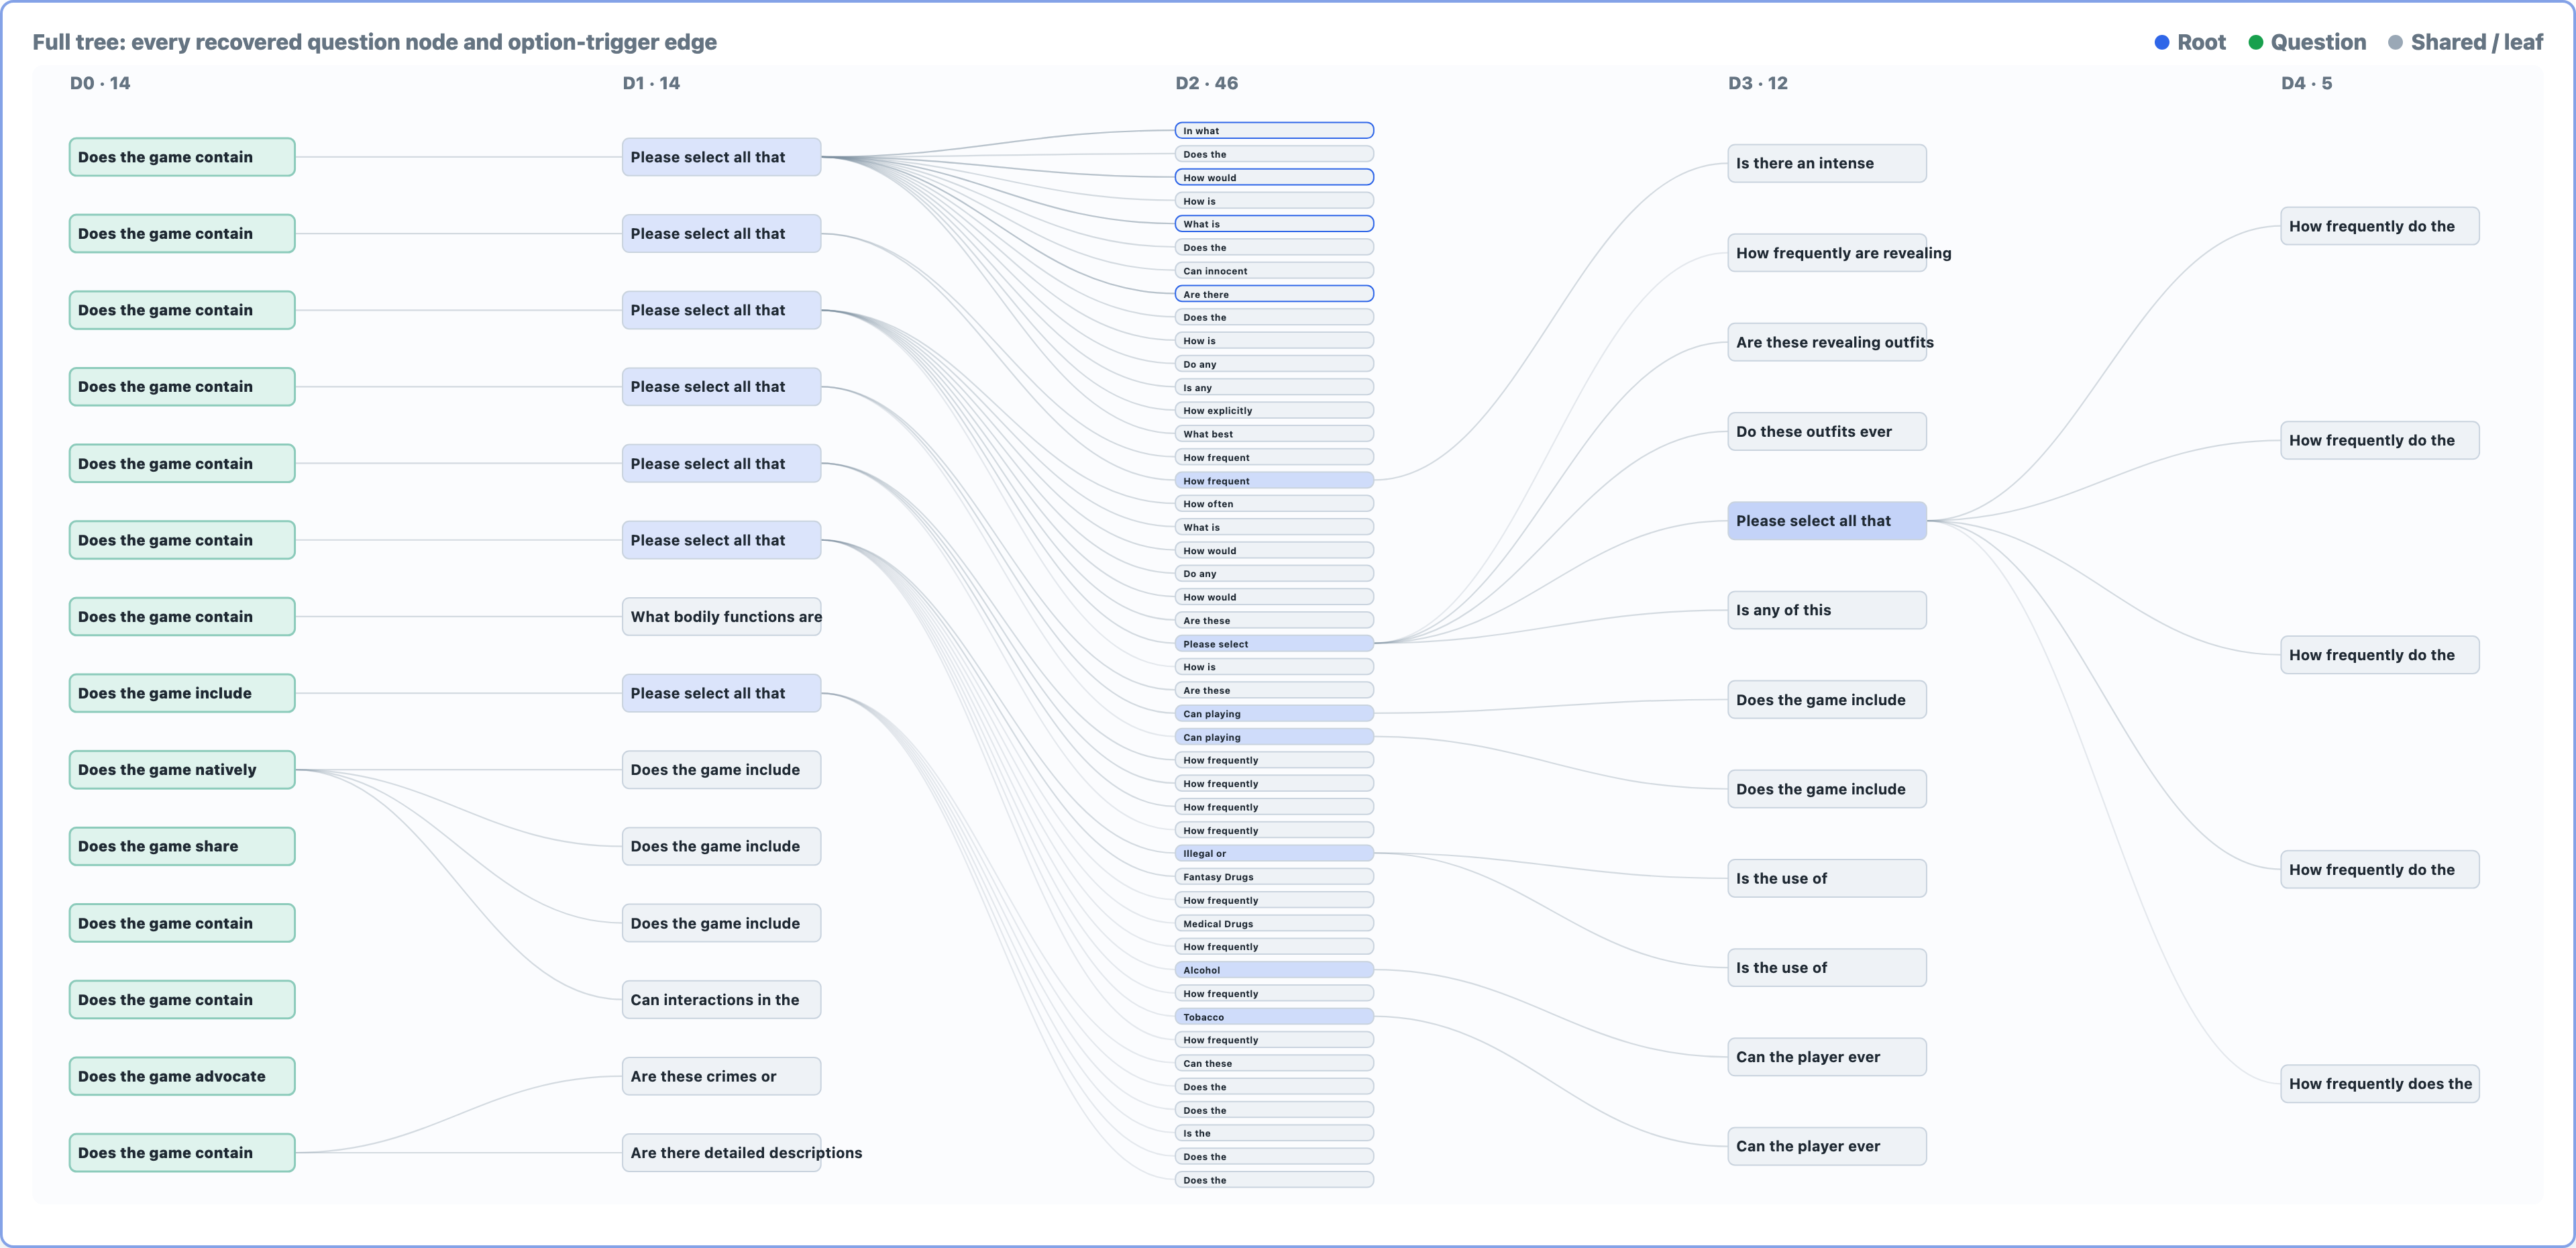
\includegraphics[width=\textwidth]{figures/game_question_graph_tree_only.png}
  \caption{Game 分类问卷结构拓扑}
  \label{fig:game-structure}
\end{subfigure}
\hfill
\begin{subfigure}{0.48\textwidth}
  \centering
  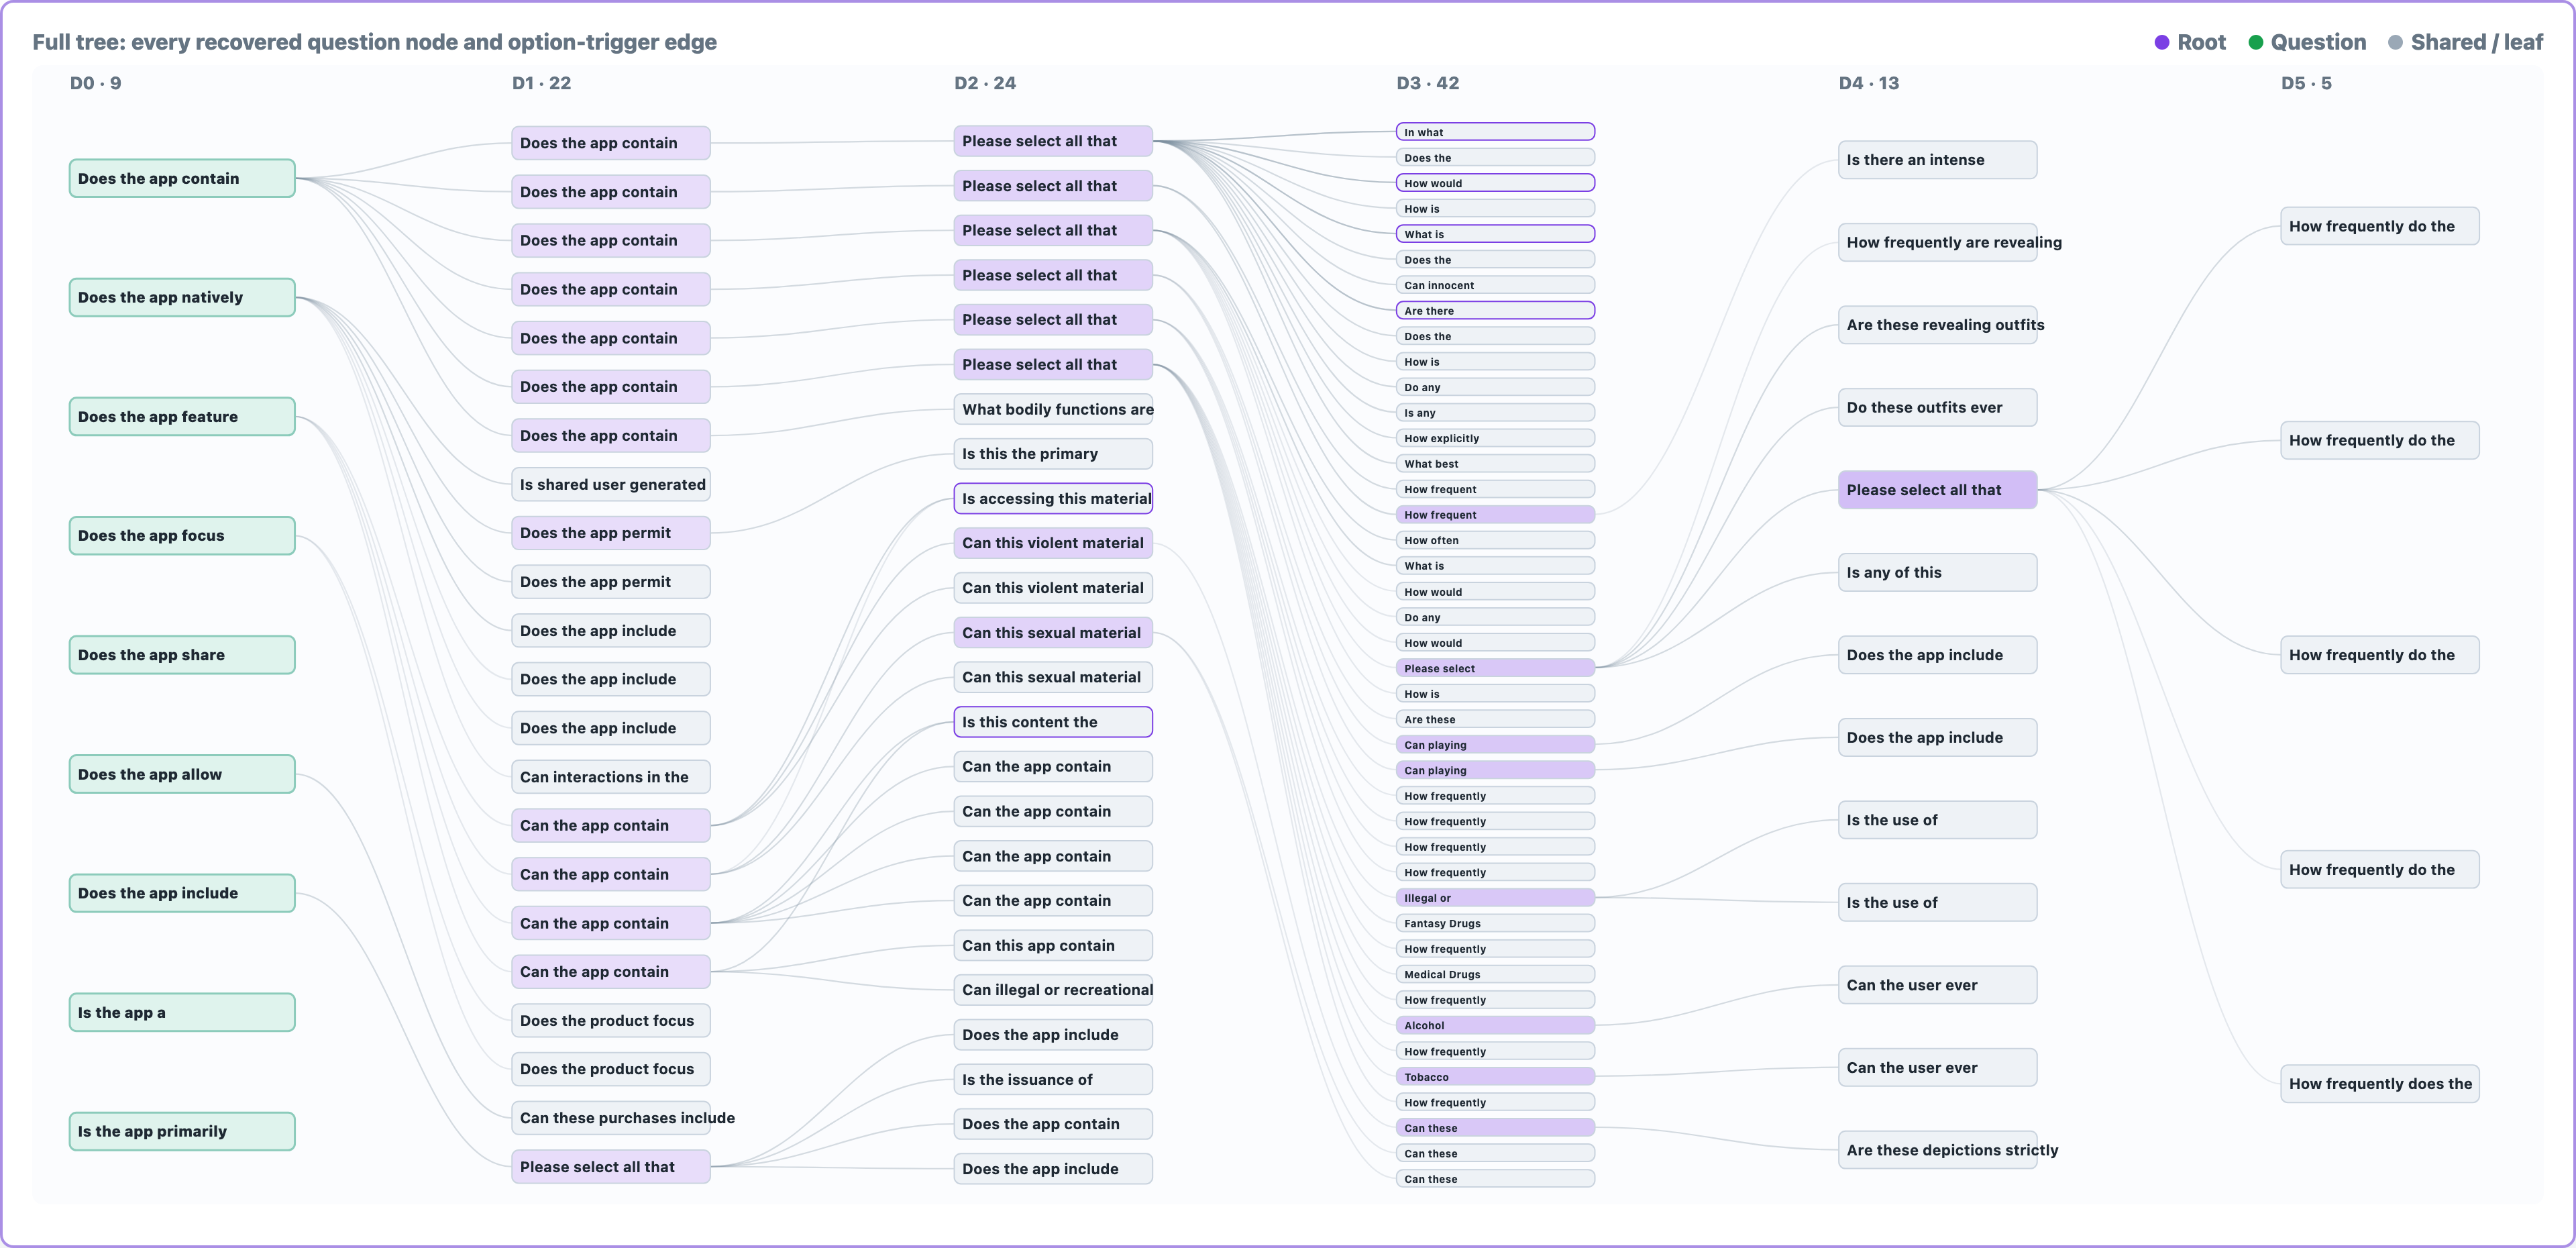
\includegraphics[width=\textwidth]{figures/all_other_question_graph_tree_only.png}
  \caption{All Other App Types 分类问卷结构拓扑}
  \label{fig:other-structure}
\end{subfigure}
\caption{自动化探测导出的两类典型问卷结构图。}
\label{fig:questionnaire-structures}
\end{figure}

\begin{figure}[H]
\centering
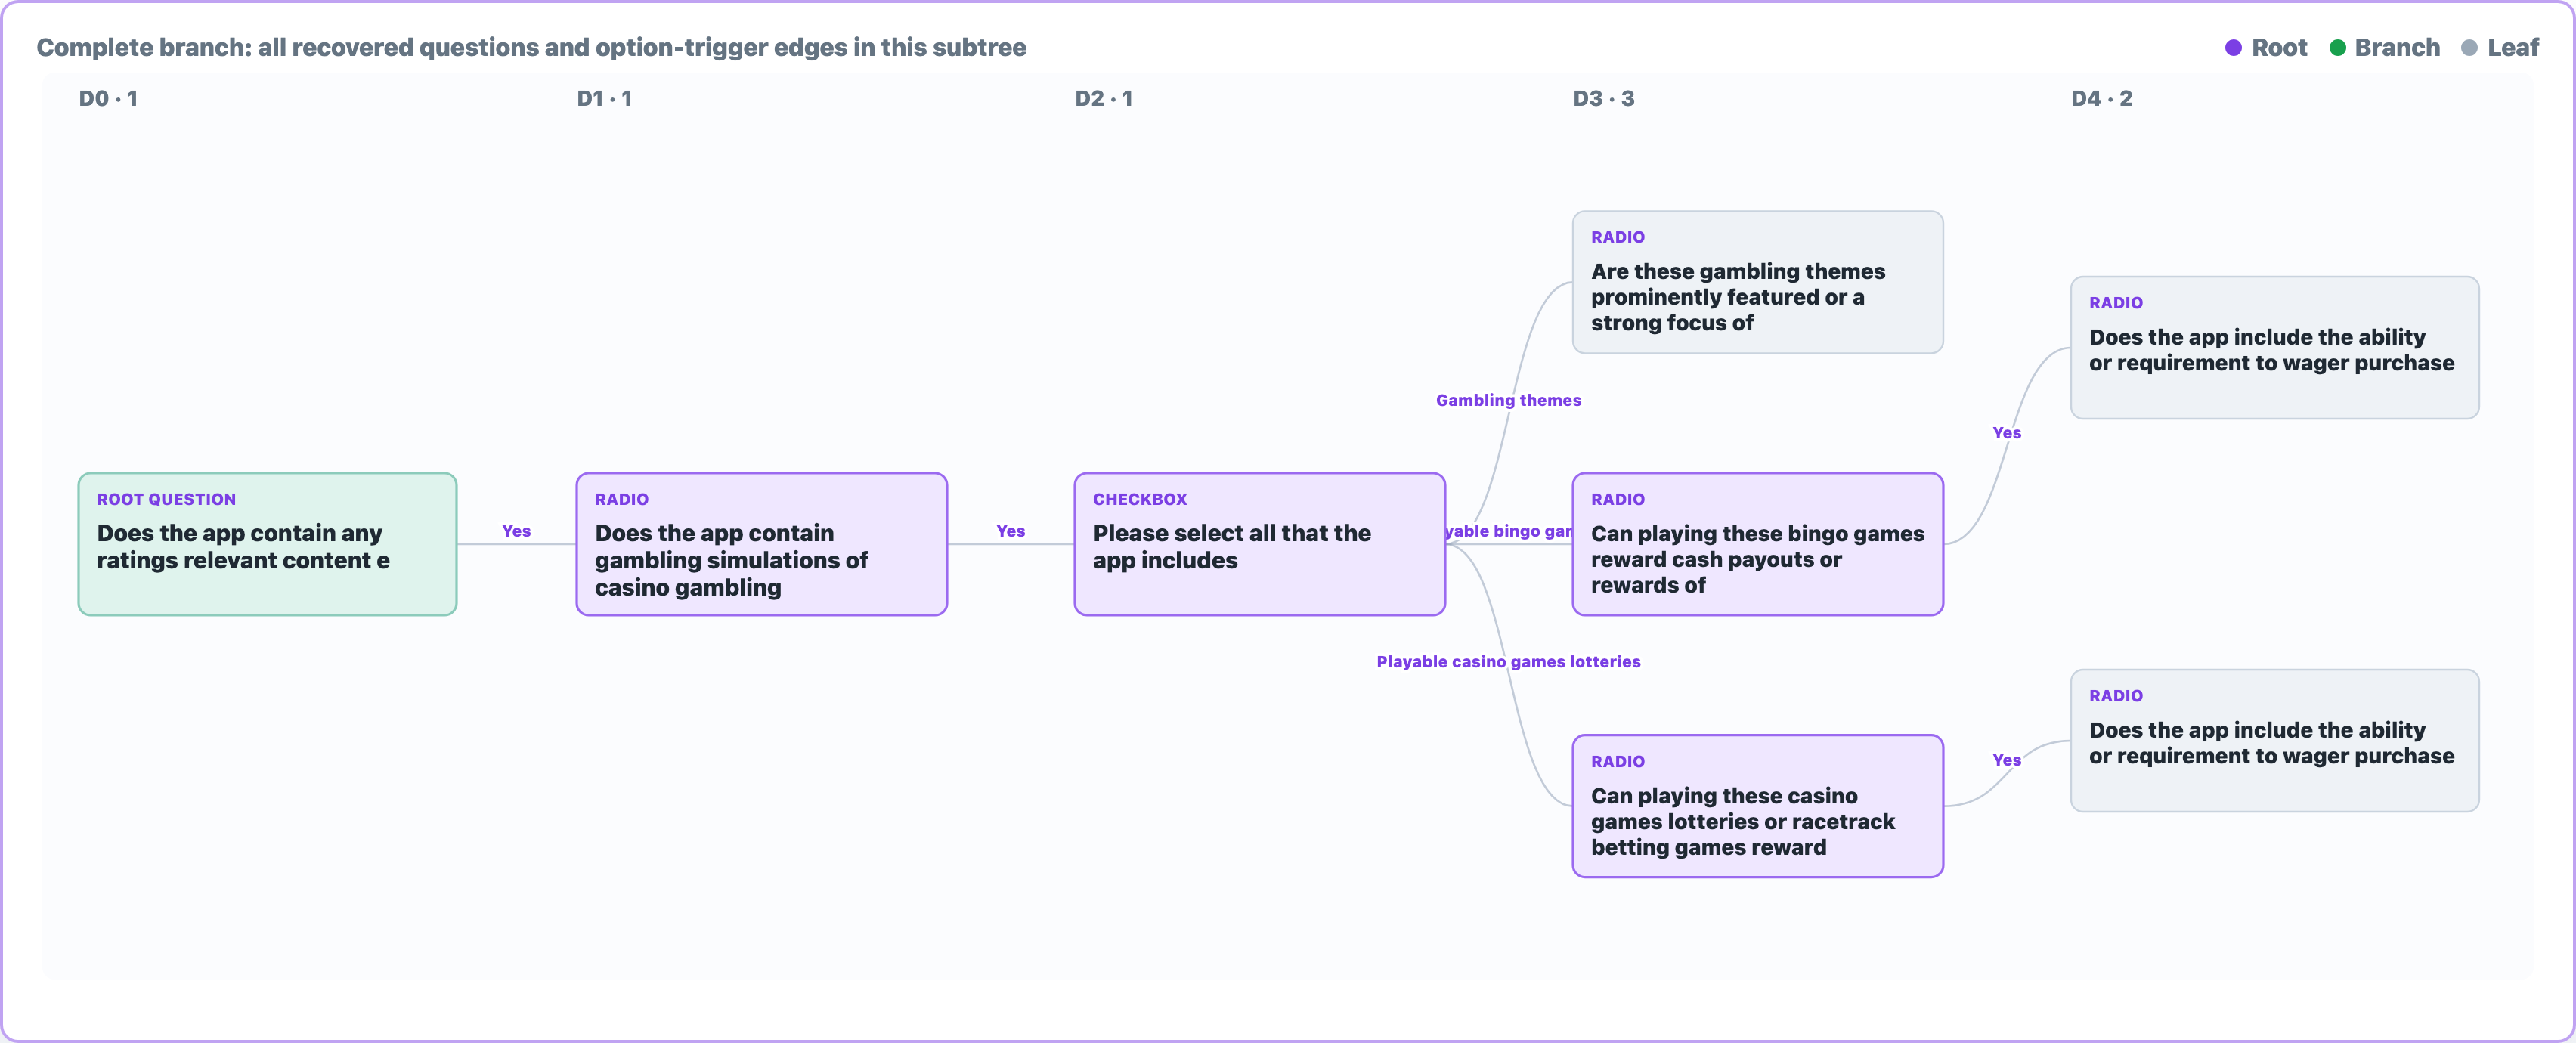
\includegraphics[width=0.72\textwidth]{figures/depth4_branch_example_content.png}
\caption{典型问题节点的局部结构与选项依赖示例（深度为4的问题分支）。}
\label{fig:question-example}
\end{figure}

本项目覆盖的应用类别包括：
\begin{itemize}[leftmargin=2em]
  \item All Other App Types；
  \item Game；
  \item Social or Communication。
\end{itemize}

不同类别对应不同问题分支。例如 Game 类更容易触发游戏内奖励、虚拟货币、赌博模拟等问题；Social or Communication 类会涉及用户生成内容、社交互动、信息共享等问题；All Other App Types 则是通用应用类别。

\subsection{采样策略}

如果对所有问题选项进行完全组合，样本空间会急剧膨胀；同时，大量组合可能只是重复低风险路径，对模型训练贡献有限。因此项目采用多层次采样策略：

\begin{enumerate}[leftmargin=2em]
  \item \textbf{Baseline 样本}：为每个类别生成低风险默认路径，用于覆盖基础问卷状态。
  \item \textbf{结构性样本}：沿问卷树分支系统性改变选项，保证不同父子依赖路径被访问。
  \item \textbf{风险样本}：针对暴力、血腥、性内容、药物、赌博、现金奖励等高风险问题生成更密集的样本。
  \item \textbf{中间带样本}：针对 Everyone 10+、Teen、Mature 17+ 等边界类别补充样本。
  \item \textbf{覆盖驱动样本}：统计低频选中选项，优先生成覆盖不足的问题选项组合。
  \item \textbf{gap-fill 样本}：对候选池中缺失或低覆盖的可达选项，直接基于问卷图生成补洞样本。
\end{enumerate}

这种策略比随机采样更适合树状问卷：一方面避免大量重复的低信息样本，另一方面能主动覆盖高风险路径与模型容易混淆的边界区域。

\section{自动化数据收集}

\subsection{自动化流程}

数据采集脚本需要在 Google Play Developer Console 中完成完整提交流程。核心步骤如下：

\begin{enumerate}[leftmargin=2em]
  \item 连接带有真实登录态的 Chrome 浏览器；
  \item 打开或恢复到内容分级问卷页面；
  \item 选择应用类别并接受条款；
  \item 按预设样本回答各个可见问题；
  \item 处理异步加载、弹窗和页面状态变化；
  \item 保存问卷并进入 Summary 页面；
  \item 解析各地区分级结果、内容描述符和互动元素；
  \item 记录结果、证据、错误和运行配置；
  \item 根据 checkpoint 继续下一批样本或重试失败样本。
\end{enumerate}

\subsection{核心自动化代码}

以下代码片段展示了项目如何复用 Chrome CDP 登录态，并优先使用已经打开的内容分级页面。这一设计避免了 Google 登录风控和账号 slot 切换问题。

\begin{lstlisting}[caption={连接真实 Chrome 并复用内容分级页面的核心逻辑}]
async function openBrowserPage() {
  const browser = await chromium.connectOverCDP(config.cdpUrl);
  const context = browser.contexts()[0] || await browser.newContext();
  const existing = context.pages().find((candidate) =>
    candidate.url().includes('/content-rating')
  );
  const page = existing || context.pages()[0] || await context.newPage();
  return {
    page,
    close: async () => {
      if (typeof browser.disconnect === 'function') browser.disconnect();
    },
  };
}
\end{lstlisting}

自动化采集脚本还实现了状态恢复逻辑。例如，当页面处于 overview、summary、loading、unknown 或 target-questionnaire 等不同状态时，脚本会通过返回、丢弃修改、重新导航等方式恢复到可填写状态。这样可以显著降低长时间采集过程中的人工干预成本。

\subsection{采集质量与失败记录}

最终清洗报告显示，项目源数据中包含 1265 条有效样本；另外，采集过程中记录了 770 次上游失败事件、30 条上游验证隔离样本和 13 条分级冲突样本。失败记录并未简单删除，而是被保存在 \code{failures.jsonl}、\code{validation_quarantine.jsonl} 和 \code{rating_conflicts.jsonl} 中，用于后续审计和改进采样脚本。

\begin{table}[H]
\centering
\caption{采集与清洗阶段数据质量概况}
\label{tab:quality}
\renewcommand{\arraystretch}{1.25}
\begin{tabular}{lr}
\toprule
项目 & 数量 \\
\midrule
清洗后有效样本 & 1265 \\
Task 3 阶段额外排除样本 & 0 \\
训练集样本 & 1012 \\
测试集样本 & 253 \\
统一问卷答案列 & 164 \\
类别-问题组合 & 218 \\
地区分级标签列 & 10 \\
上游验证隔离样本 & 30 \\
上游分级冲突样本 & 13 \\
上游失败事件 & 770 \\
\bottomrule
\end{tabular}
\end{table}

\section{数据清洗与数据集分析}

\subsection{清洗原则}

Task 3 数据清洗阶段的目标是从原始采集记录构建可用于建模的干净表格数据，同时避免任何形式的标签泄漏。清洗流程包括：

\begin{itemize}[leftmargin=2em]
  \item 验证 schema version 和必要字段；
  \item 检查 radio 选择是否合法；
  \item 检查 explicit answer 与完整问卷状态是否一致；
  \item 验证问卷图可达性，避免不可达问题状态进入数据集；
  \item 检查类别对应的地区分级数量是否符合预期；
  \item 去除重复 sample ID 和重复语义问卷状态；
  \item 排除同一问卷状态得到冲突分级的样本；
  \item 将结构性状态统一编码为非空 sentinel，避免空白单元格。
\end{itemize}

项目没有进行统计插补。原因是本任务中的“缺失”通常来自问卷分支逻辑，而不是随机缺失。例如，\code{__INACTIVE__} 表示某个问题属于该类别但未被当前父问题激活；\code{__NOT_APPLICABLE__} 表示该问题或地区分级不适用于当前类别；\code{__NONE__} 表示激活的 checkbox 问题没有选择任何选项。这些状态本身都可能携带预测信息。

\subsection{训练/测试划分}

数据集采用确定性 80/20 holdout 划分，并按应用类别与北美分级标签进行分层。固定 seed 为 \code{osn-lab2-task3-v1}。这种划分方式有两个优点：

\begin{enumerate}[leftmargin=2em]
  \item 保证各年龄分级在训练集和测试集中的比例基本一致；
  \item 保证不同运行环境下复现实验时划分结果一致。
\end{enumerate}

\begin{table}[H]
\centering
\caption{应用类别分布}
\label{tab:category-distribution}
\renewcommand{\arraystretch}{1.25}
\begin{tabular}{lrrrr}
\toprule
应用类别 & 总数 & 训练集 & 测试集 & 测试占比 \\
\midrule
All Other App Types & 616 & 492 & 124 & 20.13\% \\
Game & 633 & 507 & 126 & 19.91\% \\
Social or Communication & 16 & 13 & 3 & 18.75\% \\
\midrule
合计 & 1265 & 1012 & 253 & 20.00\% \\
\bottomrule
\end{tabular}
\end{table}

\begin{table}[H]
\centering
\caption{北美 ESRB 分级分布}
\label{tab:rating-distribution}
\renewcommand{\arraystretch}{1.25}
\begin{tabular}{lrrrr}
\toprule
年龄分级 & 总数 & 训练集 & 测试集 & 测试占比 \\
\midrule
Everyone & 182 & 146 & 36 & 19.78\% \\
Everyone 10+ & 138 & 110 & 28 & 20.29\% \\
Teen & 339 & 271 & 68 & 20.06\% \\
Mature 17+ & 365 & 292 & 73 & 20.00\% \\
Adults only 18+ & 241 & 193 & 48 & 19.92\% \\
\midrule
合计 & 1265 & 1012 & 253 & 20.00\% \\
\bottomrule
\end{tabular}
\end{table}

\subsection{数据分布可视化}

图~\ref{fig:data-bars} 用手工比例柱状图展示了不同年龄分级的样本规模。可以看到 Mature 17+ 和 Teen 样本较多，Everyone 10+ 样本最少；这会影响模型在中间类别上的召回率和 F1。

\begin{figure}[H]
\centering
\begin{tikzpicture}[x=1cm,y=0.013cm]
  \draw[->] (0,0) -- (12.7,0) node[right]{类别};
  \draw[->] (0,0) -- (0,400) node[above]{样本数};
  \foreach \y in {100,200,300,400} {
    \draw[black!15] (0,\y) -- (12.1,\y);
    \node[left] at (0,\y) {\small \y};
  }
  \def\barw{0.55}
  \foreach \x/\name/\train/\test/\total in {
    1/Everyone/146/36/182,
    3.2/Everyone 10+/110/28/138,
    5.4/Teen/271/68/339,
    7.6/Mature 17+/292/73/365,
    9.8/Adults only 18+/193/48/241
  }{
    \fill[blue!55] (\x,0) rectangle ++(\barw,\train);
    \fill[orange!75] (\x+\barw,0) rectangle ++(\barw,\test);
    \node[rotate=22, anchor=east, font=\small] at (\x+0.55,-18) {\name};
    \node[font=\scriptsize] at (\x+0.55,\total+18) {\total};
  }
  \fill[blue!55] (10.9,360) rectangle ++(0.35,18);
  \node[right, font=\small] at (11.3,369) {Train};
  \fill[orange!75] (10.9,330) rectangle ++(0.35,18);
  \node[right, font=\small] at (11.3,339) {Test};
\end{tikzpicture}
\caption{北美 ESRB 分级样本分布。数字为每个分级的总样本数。}
\label{fig:data-bars}
\end{figure}

\section{特征工程}

\subsection{输入输出定义}

本项目的预测目标为 \code{rating__north_america}，模型输入只允许使用：

\begin{itemize}[leftmargin=2em]
  \item \code{category}：应用类别；
  \item \code{answer__*}：问卷答案列。
\end{itemize}

为了防止标签泄漏，所有 \code{rating__*} 列均从特征中排除。即使我们只预测北美分级，也不能使用欧洲、德国、澳大利亚等地区分级作为输入，因为这些分级本质上也是同一次黑盒输出的一部分，使用它们会让模型得到不合理的信息优势。

\subsection{编码方案}

特征工程阶段从 Task 3 的训练集再次划分出验证集。Task 4 最终划分为：

\begin{itemize}[leftmargin=2em]
  \item 训练集：810 条；
  \item 验证集：202 条；
  \item 测试集：253 条，保持 Task 3 测试集不变。
\end{itemize}

编码方案如下：

\begin{enumerate}[leftmargin=2em]
  \item \textbf{类别与 radio 字段}：采用 one-hot 编码，每个可能取值变成一个 0/1 特征。
  \item \textbf{checkbox 字段}：按 \code{ || } 分割多选答案，再采用 multi-hot 编码。
  \item \textbf{结构性 sentinel}：\code{__INACTIVE__}、\code{__NOT_APPLICABLE__}、\code{__NONE__} 均保留为显式取值。
  \item \textbf{未知值处理}：验证集或测试集中出现训练集未见过的新答案值时，编码器忽略该值，并记录到 \code{unseen_values.json}。
\end{enumerate}

\begin{table}[H]
\centering
\caption{特征工程规模}
\label{tab:feature-scale}
\renewcommand{\arraystretch}{1.25}
\begin{tabular}{lr}
\toprule
项目 & 数量 \\
\midrule
原始特征列 & 165 \\
类别 / radio one-hot 字段 & 133 \\
checkbox multi-hot 字段 & 32 \\
编码后特征列 & 758 \\
Task 4 训练样本 & 810 \\
Task 4 验证样本 & 202 \\
最终测试样本 & 253 \\
\bottomrule
\end{tabular}
\end{table}

\subsection{特征工程核心代码}

以下代码片段展示了特征工程脚本中的几个关键设计：固定 label 顺序、结构性缺失 sentinel、确定性验证集划分。

\begin{lstlisting}[language=Python, caption={特征工程中的标签顺序与结构性状态定义}]
MISSING_SENTINELS = {"__INACTIVE__", "__NOT_APPLICABLE__", "__NONE__"}
CHECKBOX_SEPARATOR = " || "
DEFAULT_LABEL_ORDER = [
    "Everyone",
    "Everyone 10+",
    "Teen",
    "Mature 17+",
    "Adults only 18+",
]
\end{lstlisting}

\begin{lstlisting}[language=Python, caption={按 category + rating 进行确定性验证集划分}]
def deterministic_validation_split(train_df, target_column, validation_ratio, seed):
    strata = train_df["category"].astype(str) + " | " + train_df[target_column].astype(str)
    train_indices = []
    val_indices = []

    for _, group in train_df.assign(_stratum=strata).groupby("_stratum", sort=True):
        records = []
        for idx, row in group.iterrows():
            key = f"{seed}|{row['sample_id']}|{row['_stratum']}"
            records.append((stable_hash(key), idx))
        records.sort()

        n = len(records)
        if n <= 1:
            n_val = 0
        else:
            n_val = max(1, round(n * validation_ratio))
            n_val = min(n_val, n - 1)

        val_indices.extend(idx for _, idx in records[:n_val])
        train_indices.extend(idx for _, idx in records[n_val:])
\end{lstlisting}

\section{模型训练与调参}

\subsection{模型选择}

根据作业要求，项目至少需要尝试三种不同模型。我们最终训练了四类模型，以覆盖线性模型、Bagging 集成树和 Boosting 集成树：

\begin{table}[H]
\centering
\caption{模型选择与建模假设}
\label{tab:models}
\renewcommand{\arraystretch}{1.3}
\begin{tabularx}{\textwidth}{p{3.7cm}p{3.0cm}X}
\toprule
模型 & 类型 & 选择原因 \\
\midrule
Logistic Regression & 线性多分类模型 & one-hot / multi-hot 后的数据是高维稀疏特征，线性模型通常有较强基线表现；L1 正则化可自动选择关键特征。 \\
Random Forest & Bagging 集成树 & 能建模非线性特征交互，对特征缩放不敏感，适合作为树模型基线。 \\
LightGBM & Gradient Boosting & 训练速度快，适合表格数据，可通过深度、叶子数和最小叶节点样本数控制过拟合。 \\
XGBoost & Gradient Boosting & 表格任务强基线，支持列采样、早停和正则化，常用于结构化分类任务。 \\
\bottomrule
\end{tabularx}
\end{table}

\subsection{Logistic Regression 与 Random Forest}

Logistic Regression 和 Random Forest 的最终训练脚本位于 \code{task5_2_logistic_regression\&random_forest/train_models.py}。模型使用类别权重处理类别不均衡。最终参数如下：

\begin{lstlisting}[language=Python, caption={Logistic Regression 与 Random Forest 最终模型定义}]
models = {
    "logistic_regression": LogisticRegression(
        C=10.0,
        l1_ratio=1.0,
        tol=1e-4,
        solver="saga",
        max_iter=5000,
        class_weight=class_weight_by_id,
        random_state=42,
    ),
    "random_forest": RandomForestClassifier(
        n_estimators=500,
        max_depth=None,
        min_samples_leaf=1,
        max_features=0.3,
        min_samples_split=2,
        class_weight=class_weight_by_id,
        random_state=42,
        n_jobs=-1,
    ),
}
\end{lstlisting}

Logistic Regression 使用 L1 正则化，相当于在多分类权重矩阵上施加稀疏约束。由于问卷答案经 one-hot 编码后高度稀疏，L1 正则化能够自动抑制大量无关特征，保留少量对分级判定最有贡献的问题选项。

Random Forest 默认参数在本任务上表现不理想，原因之一是默认 \code{max_features='sqrt'} 在 758 维特征上每次只采样约 27 个特征，容易错过关键问卷项。调参后将 \code{max_features} 提高到 0.3，使每棵树能看到约 228 个特征，测试集 Accuracy 从约 0.617 提升到 0.783，Macro F1 从约 0.624 提升到 0.797。

\subsection{LightGBM 与 XGBoost}

LightGBM 和 XGBoost 的训练与分析位于 \code{task5_1_lightgbm\&xgboost/ana1.ipynb}。两者均采用防过拟合调参策略。

\begin{table}[H]
\centering
\caption{LightGBM 与 XGBoost 最优参数摘要}
\label{tab:gbdt-params}
\renewcommand{\arraystretch}{1.25}
\begin{tabular}{lll}
\toprule
模型 & 参数 & 最优值 / 说明 \\
\midrule
LightGBM & \code{max_depth} & 6，限制树深 \\
LightGBM & \code{num_leaves} & 15，控制叶子节点规模 \\
LightGBM & \code{min_child_samples} & 15，要求叶子至少包含较多样本 \\
LightGBM & \code{learning_rate} & 0.1 \\
\midrule
XGBoost & \code{max_depth} & 6，限制单棵树复杂度 \\
XGBoost & \code{subsample} & 1.0 \\
XGBoost & \code{colsample_bytree} & 0.8，每棵树随机选取 80\% 特征 \\
XGBoost & \code{learning_rate} & 0.1 \\
\bottomrule
\end{tabular}
\end{table}

\section{实验结果与模型对比}

\subsection{总体性能}

表~\ref{tab:model-performance} 展示了四类模型在测试集上的主要指标。整体来看，Logistic Regression 明显优于其他模型，XGBoost 次之，Random Forest 排名第三，LightGBM 表现相对较弱。

\begin{table}[H]
\centering
\caption{模型测试集性能对比}
\label{tab:model-performance}
\renewcommand{\arraystretch}{1.25}
\begin{tabular}{lccc}
\toprule
模型 & Test Accuracy & Test Macro F1 & Test Macro AUC \\
\midrule
Logistic Regression & \textbf{0.921} & \textbf{0.918} & \textbf{0.977} \\
XGBoost & 0.814 & 0.810 & 0.962 \\
Random Forest & 0.783 & 0.797 & 0.945 \\
LightGBM & 0.680 & 0.680 & 0.924 \\
\bottomrule
\end{tabular}
\end{table}

\begin{figure}[H]
\centering
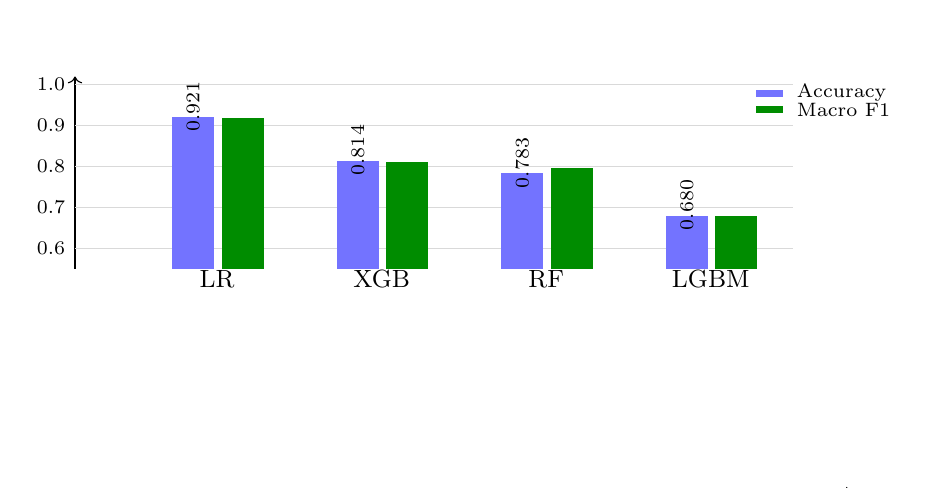
\begin{tikzpicture}[x=1.9cm,y=5.2cm]
  \draw[->] (0,0) -- (5.2,0);
  \draw[->] (0,0.55) -- (0,1.02);
  \foreach \y/\lab in {0.6/0.6,0.7/0.7,0.8/0.8,0.9/0.9,1.0/1.0} {
    \draw[black!15] (0,\y) -- (4.8,\y);
    \node[left,font=\scriptsize] at (0,\y) {\lab};
  }
  \foreach \x/\name/\acc/\f in {
    0.65/LR/0.921/0.918,
    1.75/XGB/0.814/0.810,
    2.85/RF/0.783/0.797,
    3.95/LGBM/0.680/0.680
  }{
    \fill[blue!55] (\x,0.55) rectangle ++(0.28,\acc-0.55);
    \fill[green!55!black] (\x+0.33,0.55) rectangle ++(0.28,\f-0.55);
    \node[font=\small] at (\x+0.30,0.525) {\name};
    \node[font=\scriptsize, rotate=90] at (\x+0.14,\acc+0.026) {\acc};
  }
  \fill[blue!55] (4.55,0.97) rectangle ++(0.18,0.018);
  \node[right,font=\scriptsize] at (4.76,0.979) {Accuracy};
  \fill[green!55!black] (4.55,0.93) rectangle ++(0.18,0.018);
  \node[right,font=\scriptsize] at (4.76,0.939) {Macro F1};
\end{tikzpicture}
\caption{四类模型测试集 Accuracy 与 Macro F1 对比。}
\label{fig:model-bars}
\end{figure}

\subsection{验证集与测试集泛化差距}

Logistic Regression 和 Random Forest 同时记录了验证集与测试集指标，如表~\ref{tab:val-test}。两个模型的验证集与测试集差距较小，说明不存在明显过拟合。

\begin{table}[H]
\centering
\caption{验证集与测试集表现对比}
\label{tab:val-test}
\renewcommand{\arraystretch}{1.25}
\begin{tabular}{lcccc}
\toprule
模型 & Val Accuracy & Val Macro F1 & Test Accuracy & Test Macro F1 \\
\midrule
Logistic Regression & 0.936 & 0.928 & 0.921 & 0.918 \\
Random Forest & 0.812 & 0.811 & 0.783 & 0.797 \\
\bottomrule
\end{tabular}
\end{table}

\subsection{最佳模型分类报告}

Logistic Regression 在五个 ESRB 类别上的表现如表~\ref{tab:lr-report}。可以看到 Everyone、Mature 17+、Adults only 18+ 等类别表现较好，Everyone 10+ 的 F1 相对最低，这与该类别样本较少、语义处于 Everyone 与 Teen 之间有关。

\begin{table}[H]
\centering
\caption{Logistic Regression 测试集分类报告}
\label{tab:lr-report}
\renewcommand{\arraystretch}{1.25}
\begin{tabular}{lrrrr}
\toprule
类别 & Precision & Recall & F1 & Support \\
\midrule
Everyone & 0.921 & 0.972 & 0.946 & 36 \\
Everyone 10+ & 0.889 & 0.857 & 0.873 & 28 \\
Teen & 0.855 & 0.956 & 0.903 & 68 \\
Mature 17+ & 0.957 & 0.918 & 0.937 & 73 \\
Adults only 18+ & 1.000 & 0.875 & 0.933 & 48 \\
\midrule
Macro avg & 0.924 & 0.916 & 0.918 & 253 \\
Weighted avg & 0.925 & 0.921 & 0.921 & 253 \\
\bottomrule
\end{tabular}
\end{table}

\subsection{混淆矩阵分析}

图~\ref{fig:lr-cm} 展示了 Logistic Regression 在测试集上的混淆矩阵。其主要错误集中在相邻或语义相近类别之间：

\begin{itemize}[leftmargin=2em]
  \item Everyone 10+ 中有 4 个样本被预测为 Teen；
  \item Teen 中少量样本被预测为 Everyone、Everyone 10+ 或 Mature 17+；
  \item Mature 17+ 中有 4 个样本被预测为 Teen；
  \item Adults only 18+ 中有 3 个样本被预测为 Teen、2 个样本被预测为 Mature 17+。
\end{itemize}

这说明模型错误并非随机分散，而是主要发生在年龄分级边界附近。

\begin{figure}[H]
\centering
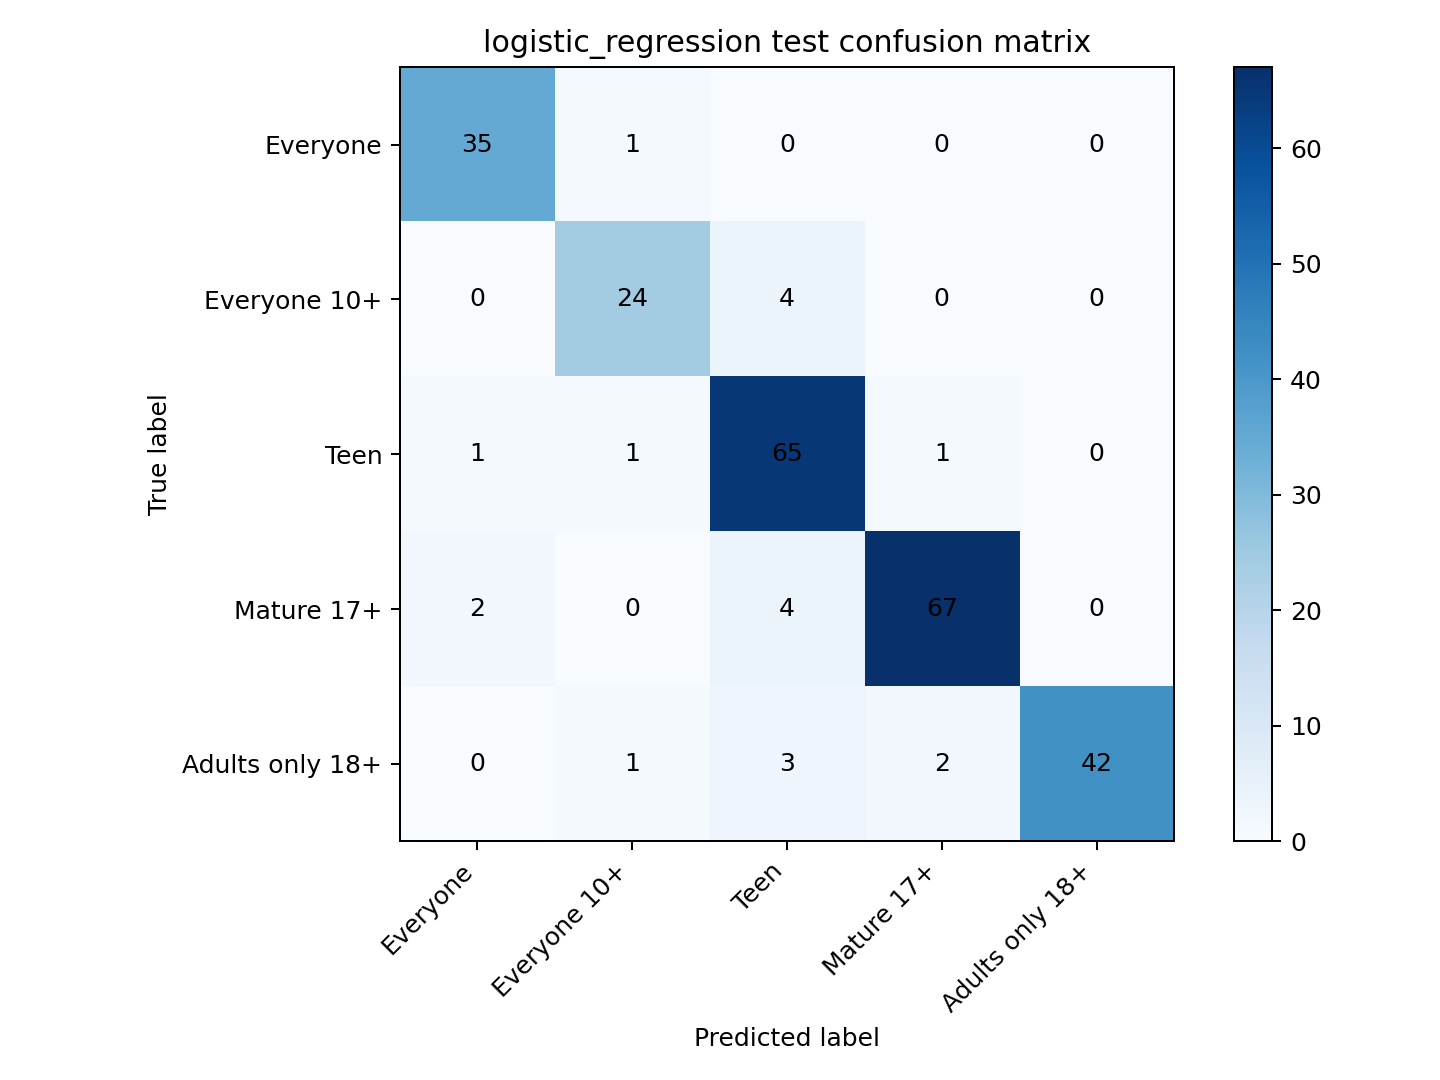
\includegraphics[width=0.72\textwidth]{figures/confusion_matrix_logistic_regression_test.png}
\caption{Logistic Regression 测试集混淆矩阵。}
\label{fig:lr-cm}
\end{figure}

Random Forest 的混淆矩阵如图~\ref{fig:rf-cm}。相比 Logistic Regression，Random Forest 对 Teen 与 Mature 17+ 的区分更弱，Mature 17+ 被预测为 Teen 的比例更高。这反映出在小规模高维稀疏数据上，树模型需要更多样本才能稳定学习到细粒度边界。

\begin{figure}[H]
\centering
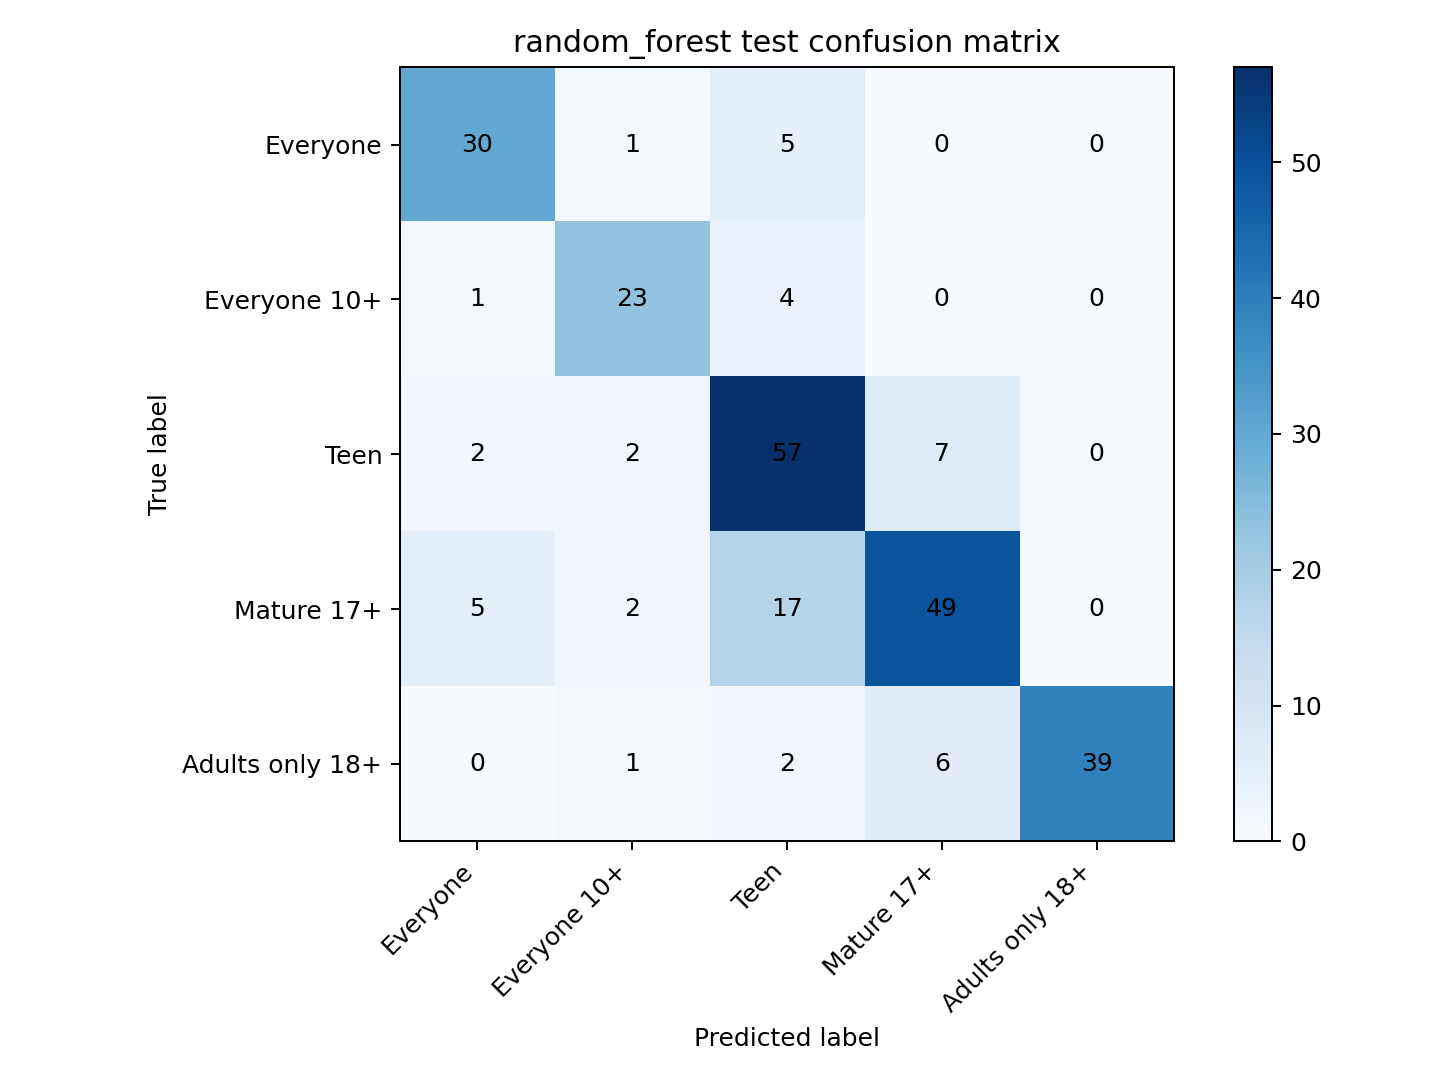
\includegraphics[width=0.72\textwidth]{figures/confusion_matrix_random_forest_test.png}
\caption{Random Forest 测试集混淆矩阵。}
\label{fig:rf-cm}
\end{figure}

\begin{figure}[H]
\centering
\begin{subfigure}{0.48\textwidth}
  \centering
  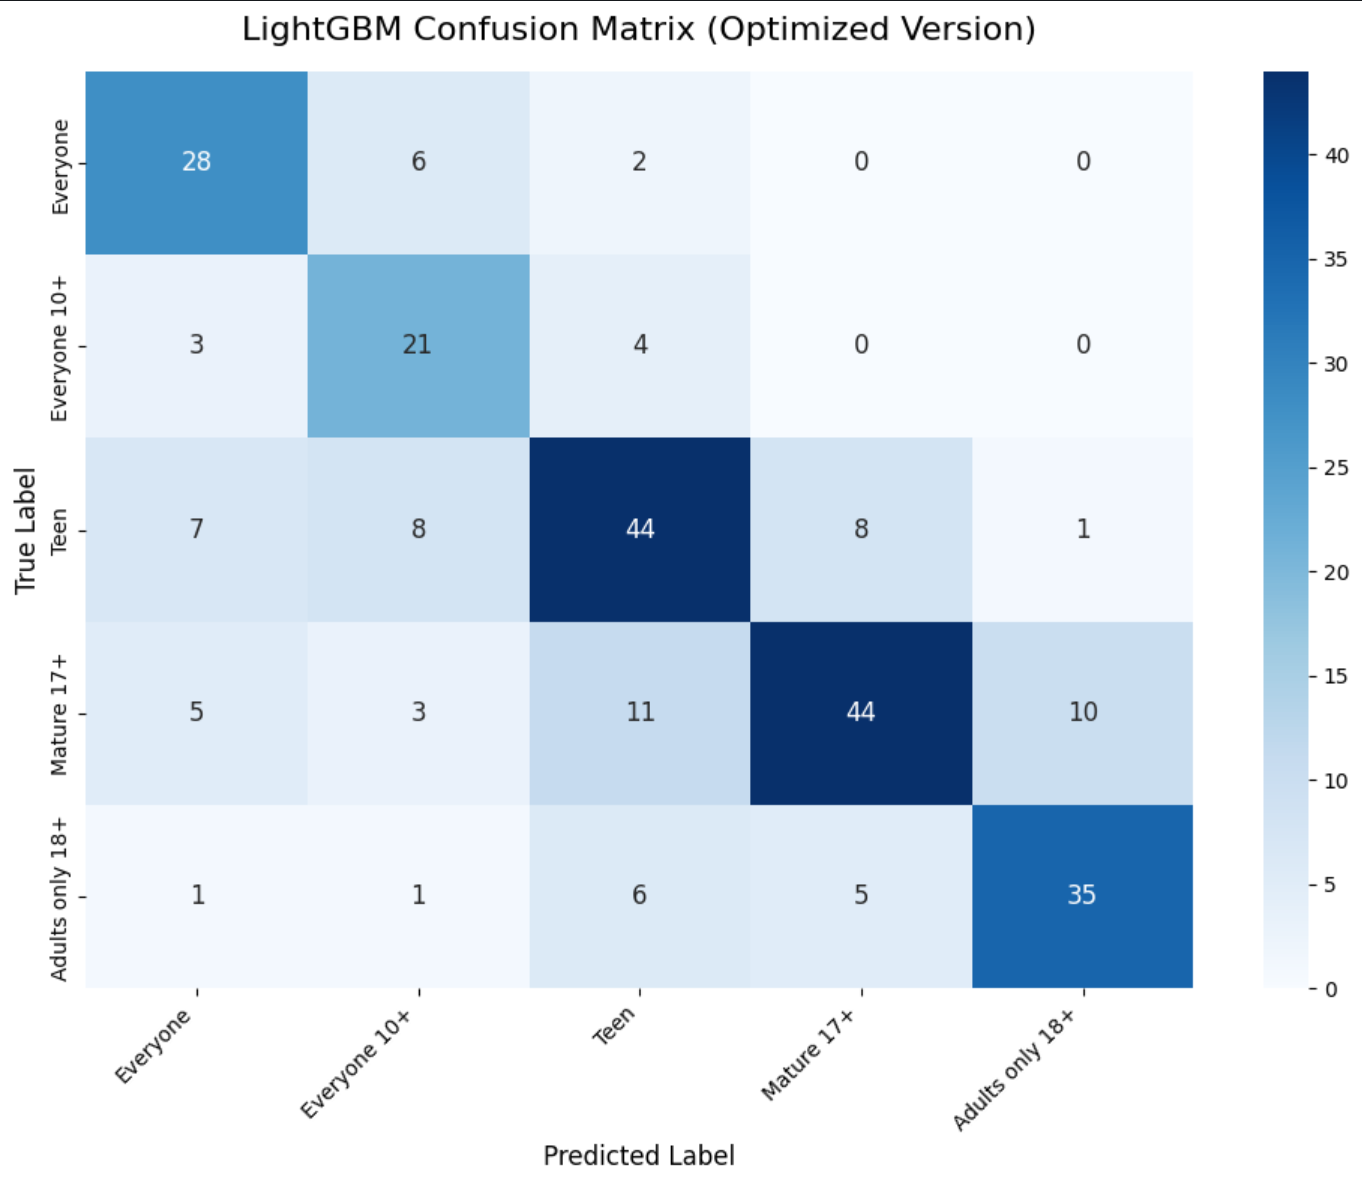
\includegraphics[width=\textwidth]{figures/lightgbm.png}
  \caption{LightGBM}
\end{subfigure}
\hfill
\begin{subfigure}{0.48\textwidth}
  \centering
  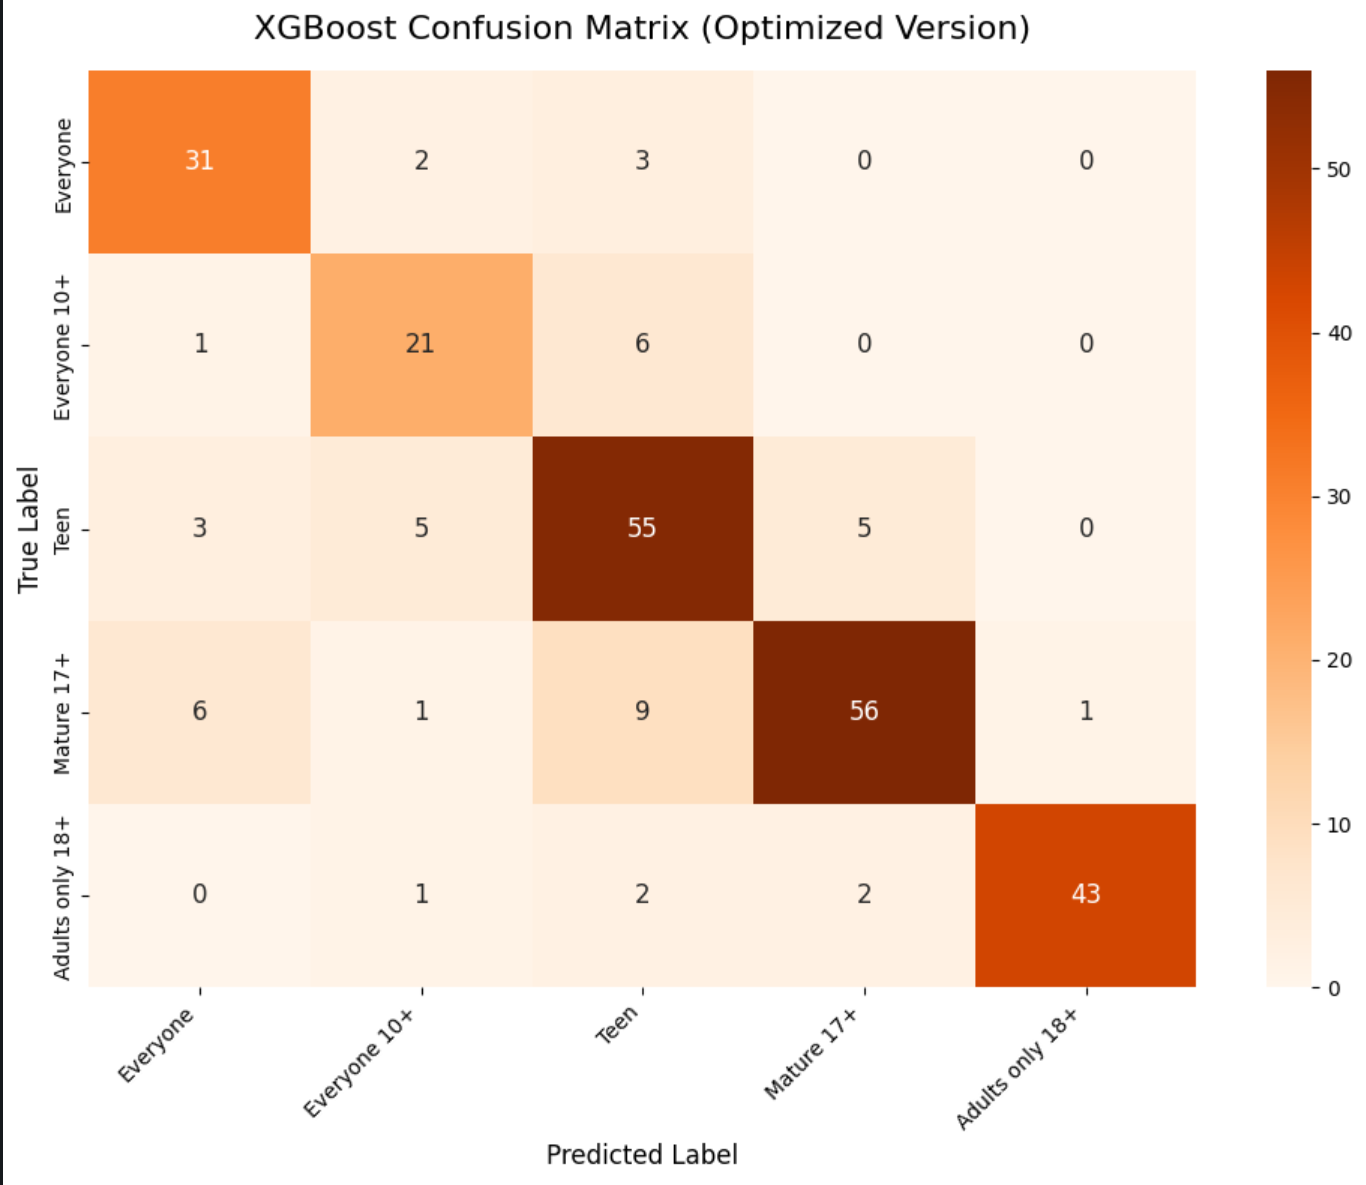
\includegraphics[width=\textwidth]{figures/xgboost.png}
  \caption{XGBoost}
\end{subfigure}
\caption{LightGBM 与 XGBoost 测试集混淆矩阵。XGBoost 整体优于 LightGBM，但仍低于 L1 Logistic Regression。}
\label{fig:gbdt-cm}
\end{figure}

\section{深入分析}

\subsection{为什么 L1 Logistic Regression 表现最好}

本项目最重要的实验现象是：相对更简单的 L1 Logistic Regression 击败了 Random Forest、LightGBM 和 XGBoost。这一结果并不矛盾，原因在于本任务的特征形态与线性稀疏模型高度匹配。

问卷答案经过 one-hot 和 multi-hot 编码后形成 758 维稀疏特征。每个样本只会激活少量特征，多数特征为 0。Google Play 分级规则很可能近似由若干强触发条件叠加构成，例如“高等级血腥内容”“性器官出现频繁”“赌博与现金奖励”等答案会显著提高年龄分级。这种规则在 one-hot 空间中往往接近线性可分或分段线性可分。

L1 正则化的优势包括：

\begin{enumerate}[leftmargin=2em]
  \item \textbf{适配高维稀疏数据}：L1 正则化会将大量无关特征权重压缩为 0。
  \item \textbf{降低过拟合风险}：在 1265 条样本和 758 维特征的比例下，稀疏约束能显著减少有效参数。
  \item \textbf{保留可解释性}：每个非零系数都对应具体问题选项，便于分析分级机制。
  \item \textbf{捕捉强单因素规则}：如果某些选项本身就足以决定分级，线性模型能够直接学习到高权重。
\end{enumerate}

相比之下，树模型在高维稀疏 one-hot 特征上需要通过大量轴对齐分裂捕捉相同规则。当样本量不足或某些类别样本稀少时，树模型更容易受到稀疏特征噪声影响。LightGBM 的叶子生长策略在小样本稀疏矩阵上尤其容易受到参数约束影响，导致欠拟合或不稳定。

\subsection{核心影响因素}

根据仓库中已有分析，SHAP 与 L1 系数共同指向以下高影响因素：

\begin{table}[H]
\centering
\caption{影响 Google Play 年龄分级的主要问卷信号}
\label{tab:important-features}
\renewcommand{\arraystretch}{1.25}
\begin{tabularx}{\textwidth}{p{1.2cm}p{6.2cm}X}
\toprule
排名 & 影响因素 & 解释 \\
\midrule
1 & 血液/血腥程度 & 血腥程度越高，越容易推向 Teen、Mature 17+ 或 Adults only 18+。 \\
2 & 生殖器或性内容出现频率 & 性内容是 ESRB 高年龄分级的重要触发因素，频率和显性程度会影响标签边界。 \\
3 & 色情/挑逗性场景分支 & 是否进入相关分支本身就是风险信号；未激活状态也可能帮助模型判断低风险。 \\
4 & 非法或娱乐性药物引用 & 药物相关内容通常会提高分级，尤其影响 Teen 与 Mature 17+ 边界。 \\
5 & 赌博、现金奖励、模拟赌博 & 涉及真钱、现金奖励或赌博模拟时，分级可能显著提高。 \\
6 & 用户交互与内容共享 & 对 Social or Communication 类尤其重要，但当前样本较少，结论需谨慎。 \\
\bottomrule
\end{tabularx}
\end{table}

这些因素与常识中的年龄分级原则一致：越涉及暴力、血腥、性、毒品、赌博、金钱奖励等内容，应用越可能获得更高年龄限制。

\subsection{结构性缺失值的意义}

传统表格任务常把缺失值视为需要填充的噪声，但本项目中 \code{__INACTIVE__}、\code{__NOT_APPLICABLE__} 和 \code{__NONE__} 都是问卷逻辑的一部分。尤其是 \code{__INACTIVE__}，它表示某个问题由于父问题选择而没有出现。例如，如果一个血腥内容子问题没有被激活，可能说明父问题选择了“不包含血腥内容”；这显然是预测低年龄分级的重要信息。

因此，项目没有采用均值填充、众数填充等统计插补，而是将这些结构性状态作为普通类别值进行 one-hot 编码。这一选择在后续模型解释中得到支持：\code{__INACTIVE__} 多次出现在重要特征列表中，说明问卷的“未触发路径”与“触发路径”一样具有信息量。

\subsection{问卷冗余与关键特征}

仓库分析指出，按 L1 系数绝对值排序后，仅使用部分高权重特征即可接近甚至超过全量特征表现：

\begin{table}[H]
\centering
\caption{特征数量与测试集 Accuracy 的关系}
\label{tab:feature-redundancy}
\renewcommand{\arraystretch}{1.25}
\begin{tabular}{rrr}
\toprule
使用特征数 & Test Accuracy & 相对全量性能 \\
\midrule
10 & 0.435 & 47\% \\
50 & 0.625 & 68\% \\
200 & 0.933 & 101\% \\
758 & 0.921 & 100\% \\
\bottomrule
\end{tabular}
\end{table}

这说明 Google Play 问卷中存在较强冗余。大量问题或选项对北美 ESRB 分级贡献有限，或者只在非常少数的边界场景中起作用。对于黑盒逆向建模而言，这一发现有两个意义：

\begin{enumerate}[leftmargin=2em]
  \item 可以用较少关键问题构造近似预测器，降低填写和建模成本；
  \item 可以反向推断分级机制中的高权重规则，帮助开发者理解哪些内容风险最需要关注。
\end{enumerate}

\subsection{分级边界的灰色地带}

模型最不确定的样本集中在中间类别边界，尤其是 Teen 与 Mature 17+、Everyone 10+ 与 Teen 之间。这与 ESRB 分级本身的语义有关：Everyone 与 Adults only 18+ 往往对应非常低风险或非常高风险内容，边界相对清晰；而 Everyone 10+、Teen、Mature 17+ 则涉及风险程度、出现频率、表现方式等细粒度差异。

从混淆矩阵可以看出，Logistic Regression 很少将 Everyone 直接预测为 Adults only 18+，也很少将 Adults only 18+ 预测为 Everyone。错误主要发生在相邻类别或相近风险类别之间。这说明模型学到的年龄分级顺序基本合理。

\section{实验问题与解决方案}

\subsection{数据采集阶段问题}

\begin{longtable}{p{4.0cm}p{5.0cm}p{5.5cm}}
\caption{数据采集阶段问题与解决方案}
\label{tab:collection-problems}\\
\toprule
问题 & 影响 & 解决方案 \\
\midrule
\endfirsthead
\toprule
问题 & 影响 & 解决方案 \\
\midrule
\endhead
Google 登录风控 & Playwright 默认浏览器可能无法登录 Google 账号，导致无法访问 Developer Console。 & 改用真实 Chrome profile，并通过 CDP 连接已登录浏览器。 \\
账号 slot 切换 & Google URL 中的 \code{/u/0}、\code{/u/2} 可能对应不同账号，错误账号无权限访问页面。 & 脚本优先复用当前已打开的 content-rating 页面，并允许通过 \code{PLAY_CONSOLE_URL} 指定工作 URL。 \\
页面异步保存状态不稳定 & 保存后可能长时间 loading 或未进入 Summary 页面，导致解析不到分级结果。 & 不依赖固定等待时间，增加状态检测、重试和恢复逻辑。 \\
弹窗与模态框遮挡 & 自动点击问题选项或 Next 按钮时可能失败。 & 增加 \code{dismissOverlays}，自动按 Escape 并尝试关闭弹窗。 \\
父子依赖不满足 & 生成样本可能请求一个不可见子问题，导致填写失败。 & 采样前基于 question graph 验证可达路径，并在 gap-fill 生成中补齐激活路径。 \\
重复与冲突样本 & 同一语义状态可能重复出现，或少数状态得到冲突分级。 & 数据构建阶段语义去重，并将冲突样本写入 \code{rating_conflicts.jsonl} 排除。 \\
\bottomrule
\end{longtable}

\subsection{建模阶段问题}

\begin{table}[H]
\centering
\caption{建模阶段问题与解决方案}
\label{tab:model-problems}
\renewcommand{\arraystretch}{1.25}
\begin{tabularx}{\textwidth}{p{4.0cm}X X}
\toprule
问题 & 影响 & 解决方案 \\
\midrule
类别不均衡 & Everyone 10+ 样本最少，模型容易偏向 Teen 和 Mature 17+。 & 使用 \code{class_weight='balanced'} 或等价类别权重，提高少数类别权重。 \\
目标泄漏风险 & 其他地区 \code{rating__*} 标签与北美标签高度相关，若作为特征会虚高。 & 明确排除所有 \code{rating__*} 列，只使用 \code{category} 和 \code{answer__*}。 \\
高维稀疏特征 & 树模型默认参数可能看不到足够关键特征，导致性能偏低。 & 对 Random Forest 调大 \code{max_features}，对 boosting 模型限制深度并使用列采样。 \\
LightGBM 欠拟合 & 在本数据规模下测试集 F1 仅约 0.680。 & 尝试防过拟合调参；最终将其作为对比模型，结论中解释模型与特征形态不完全匹配。 \\
中间类别边界模糊 & Everyone 10+、Teen、Mature 17+ 更容易混淆。 & 使用 Macro F1 观察各类别公平表现，并结合混淆矩阵做边界分析。 \\
\bottomrule
\end{tabularx}
\end{table}

\section{小组分工}

由于项目跨越网页自动化、数据工程、特征工程、模型训练和报告整理多个环节，小组采用模块化协作方式推进。结合仓库任务模块与实验流程，本报告整理分工如表~\ref{tab:division}。

\begin{table}[H]
\centering
\caption{小组成员分工}
\label{tab:division}
\renewcommand{\arraystretch}{1.35}
\begin{tabularx}{\textwidth}{p{2.2cm}X}
\toprule
成员 & 主要负责内容 \\
\midrule
陈宇涵 & 项目仓库维护； Google Play Developer Console 自动化流程搭建；问卷结构探测、样本抓取与维护 \\
史家顺 & 负责把原始采集数据变成干净数据集：去重、缺失处理、异常样本筛掉、统一字段名、生成 train.csv / test.csv。 \\
陈博凡 & 特征工程模块；整理原始问卷字段、结构性缺失 sentinel、one-hot / multi-hot 编码方案，输出特征字典、标签映射和预处理器。 \\
陈子涵 & LightGBM 与 XGBoost 模型训练和调参；完成 boosting 模型实验、混淆矩阵绘制、模型对比与补充分析。 \\
王子轩 & Logistic Regression 与 Random Forest 模型训练；完成类别权重、参数搜索、模型保存、分类报告和混淆矩阵输出。 \\
\bottomrule
\end{tabularx}
\end{table}

实际协作中，各模块之间存在交叉。例如数据采集结果会反向影响特征工程，模型混淆矩阵又会提示哪些问卷分支需要补采样。因此，上述分工并不是割裂的流水线，而是围绕共同目标形成的协作闭环。

\section{项目主要发现}

综合数据、模型和解释分析，本项目得到以下结论：

\begin{enumerate}[leftmargin=2em]
  \item \textbf{Google Play 年龄分级问卷可以被较高准确率逆向预测。} 在 1265 条有效样本上，L1 Logistic Regression 测试集 Accuracy 达到 0.921，Macro F1 达到 0.918，说明问卷答案与北美 ESRB 分级之间存在稳定可学习的映射关系。
  \item \textbf{高维稀疏问卷数据更适合稀疏线性模型。} 尽管 Random Forest、LightGBM、XGBoost 都是强表格模型，但本任务中 L1 正则化 Logistic Regression 表现最佳，说明规则型问卷映射更接近稀疏线性触发机制。
  \item \textbf{暴力/血腥、性内容、药物、赌博是最核心的风险信号。} 这些问题对年龄分级影响最大，符合 ESRB 内容分级的常识。
  \item \textbf{问卷分支结构本身携带信息。} \code{__INACTIVE__} 等结构性状态不应被当作普通缺失值填充，而应保留为模型特征。
  \item \textbf{问卷存在明显冗余。} 只使用约 200 个高权重特征即可接近全量 758 维特征性能，说明大量问题对北美分级预测贡献有限。
  \item \textbf{中间分级天然更难。} Everyone 10+、Teen、Mature 17+ 的边界更模糊，模型错误也主要集中在这些相邻类别之间。
\end{enumerate}

\section{局限性与改进方向}

\subsection{当前局限性}

\begin{enumerate}[leftmargin=2em]
  \item \textbf{Social or Communication 样本过少}：该类别只有 16 条样本，其中测试集仅 3 条，因此无法对该类别单独给出可靠结论。
  \item \textbf{样本规模仍有限}：虽然满足 1000 条要求，但对于包含 758 维特征和大量分支组合的问卷系统，1265 条样本仍然偏少。
  \item \textbf{黑盒系统可能随时间变化}：Google Play 或 IARC 问卷规则可能更新，当前模型只反映采集时刻的黑盒行为。
  \item \textbf{模型主要预测北美分级}：仓库保留了其他地区分级标签，但本报告主要分析 \code{rating__north_america}，尚未系统比较不同地区规则差异。
  \item \textbf{模型解释依赖相关性}：L1 系数和 SHAP 能揭示统计影响因素，但不能完全证明 Google 内部规则的因果结构。
\end{enumerate}

\subsection{后续改进方向}

后续可以从以下方向继续扩展：

\begin{itemize}[leftmargin=2em]
  \item 增加 Social or Communication 类别采样，补齐当前最薄弱的类别；
  \item 使用主动学习策略，让模型优先请求当前最不确定或最可能改变边界的样本；
  \item 对不同地区分级分别建模，比较 ESRB、PEGI、USK、ACB 等体系之间的规则差异；
  \item 构造可解释规则集，例如从 L1 高权重特征中抽取近似决策规则；
  \item 尝试校准模型概率，用于给开发者提供“不确定性提示”而不仅是单一预测标签；
  \item 将采样脚本封装为更稳定的可复现实验 pipeline，减少对交互式 Chrome 状态的依赖。
\end{itemize}

\section{结论}

本项目完整实现了 Google Play 年龄分级问卷的黑盒逆向建模流程。我们从动态问卷结构探测出发，设计多层次采样策略，通过 Playwright 与真实 Chrome CDP 自动化完成问卷提交和结果解析，最终构建了 1265 条有效样本的数据集。在严格防止标签泄漏的前提下，项目将 165 个原始输入字段编码为 758 维稀疏特征，并训练比较了 Logistic Regression、Random Forest、LightGBM 和 XGBoost 四种模型。

实验结果表明，L1 正则化 Logistic Regression 是本任务中的最优模型，在测试集上达到 0.921 Accuracy、0.918 Macro F1 和 0.977 Macro AUC。该结果说明 Google Play 年龄分级机制虽然不公开，但其输入输出关系可以被数据驱动方法较高精度地近似学习。进一步分析表明，血腥/暴力、性内容、药物、赌博等问题是影响分级的核心因素；问卷的结构性缺失状态同样包含重要信号；中间年龄分级边界存在天然模糊性。

总体而言，本项目完成了课程要求中的数据采集、特征工程、多模型预测、性能比较、结果分析和完整报告撰写，并从工程实现和模型解释两个角度展示了对黑盒分级机制的理解。

\appendix
\section{复现实验命令}

\begin{lstlisting}[language=bash, caption={项目主要复现命令}]
# 安装 Node 依赖
npm install

# 探测问卷结构
CDP_URL="http://127.0.0.1:9222" npm run inspect:questionnaire

# 运行采样
CDP_URL="http://127.0.0.1:9222" npm run run:samples

# 构建和验证 Dataset V2
npm run build:dataset-v2
npm run validate:dataset-v2

# 特征工程
python task4_feature_engineering/scripts/build_features.py

# 训练 Logistic Regression 和 Random Forest
python "task5_2_logistic_regression&random_forest/train_models.py"
\end{lstlisting}

\section{关键输出文件}

\small
\begin{longtable}{p{6.2cm}p{8.4cm}}
\caption{关键输出文件清单}
\label{tab:outputs}\\
\toprule
文件 & 内容 \\
\midrule
\endfirsthead
\toprule
文件 & 内容 \\
\midrule
\endhead
\code{dataset_v2/samples.jsonl} & 语义去重后的主样本数据。 \\
\code{dataset_v2/}\\\code{coverage_report.json} & 类别、分级、选项频率、重复和冲突统计。 \\
\code{task3_data_cleaning/}\\\code{output/clean_dataset.csv} & 清洗后的完整表格数据。 \\
\code{task3_data_cleaning/}\\\code{output/train.csv} & Task 3 训练集。 \\
\code{task3_data_cleaning/}\\\code{output/test.csv} & Task 3 测试集。 \\
\code{task4_feature_engineering/}\\\code{output/X_train.npz} & 稀疏训练特征矩阵。 \\
\code{task4_feature_engineering/}\\\code{output/feature_dictionary.csv} & 编码后特征与原始问题、选项的对应关系。 \\
\code{task4_feature_engineering/}\\\code{output/label_mapping.json} & 标签到整数 ID 的映射。 \\
\code{task5_2_logistic_regression}\\\code{\&random_forest/output/}\\\code{model_comparison.csv} & Logistic Regression 与 Random Forest 的指标汇总。 \\
\code{task5_2_logistic_regression}\\\code{\&random_forest/output/}\\\code{metrics.json} & 模型参数和验证/测试指标。 \\
\code{task5_2_logistic_regression}\\\code{\&random_forest/output/*.png} & 混淆矩阵图。 \\
\code{task5_1_lightgbm\&xgboost/}\\\code{img/*.png} & LightGBM 与 XGBoost 混淆矩阵图。 \\
\bottomrule
\end{longtable}
\normalsize

\section{参考资料}

\begin{enumerate}[leftmargin=2em]
  \item Google Play Developer Console: \url{https://play.google.com/console/developers}
  \item 项目仓库：\url{https://github.com/CYH0415/OSN-Lab-Main}
  \item Playwright Documentation: \url{https://playwright.dev/}
  \item scikit-learn Documentation: \url{https://scikit-learn.org/}
  \item XGBoost Documentation: \url{https://xgboost.readthedocs.io/}
  \item LightGBM Documentation: \url{https://lightgbm.readthedocs.io/}
\end{enumerate}

\label{LastPage}
\end{document}
